\chapter{Crop development and growth}

\section{Overview of the crop growth model}

The WOFOST model describes phenological development, growth and yield formation of
a crop from emergence till maturity on the basis of crop genetic properties and 
environmental conditions. The model simulates dry matter accumulation of a crop as a function
of irradiation, temperature and crop characteristics in time steps of one day. 
The basis for calculating dry matter production, is the rate of gross CO$_{{\rm 2}}$ assimilation of
the canopy. This rate is dependent on the radiation energy absorbed by the canopy, which
is a function of incoming radiation and of crop leaf area. From the absorbed radiation and
the photosynthetic characteristics of single leaves, the daily rate of CO$_{{\rm 2}}$ assimilation of the
crop is calculated. Part of the carbohydrates produced (CH$_{{\rm 2}}$O) are used to provide energy
for the maintenance of the existing live biomass (maintenance respiration). The remaining
carbohydrates are converted into structural matter. In this conversion, some of the weight
is lost as growth respiration. The growth rate is thus obtained as:

\begin{equation}
% eq 5.1
\Delta W ~=~ C _{e} ~( A ~-~ R _{m} )
\end{equation}

Where:\\[5pt]
\begin{tabularx}{\textwidth}{llXr}
	$\Delta$W &:& Growth rate    &   
	[kg Dry Matter ha$^{{\rm -1}}$ d$^{{\rm -1}}$]\\
	A  &:& Gross assimilation   rate &  
	[kg CH$_{{\rm 2}}$O ha$^{{\rm -1}}$ d$^{{\rm -1}}$]\\
	R$_{{\rm m}}$  &:& Maintenance respiration rate    &  
	[kg CH$_{{\rm 2}}$O ha$^{{\rm -1}}$ d$^{{\rm -1}}$]\\
	C$_{{\rm e}}$ &:& Conversion efficiency off assimilates total crop   &   
	[kg Dry Matter kg$^{{\rm -1}}$ CH$_{{\rm 2}}$O]\\
\end{tabularx}

The dry matter produced is partitioned amongst the various plant organs such as roots,
leaves, stems and storage organs, using partitioning factors that are a function of the
phenological development stage of the crop (Spitters et al., 1989). The fraction partitioned
to the leaves, determines leaf area development and hence the dynamics of light interception. 
The dry weights of the plant organs are obtained by integrating their growth rates over time.

Leaf mass is subdivided into age classes. During the development of the crop a part of
living biomass dies due to senescence. Some simulated crop growth processes are
influenced by temperature, like for example the maximum rate of photosynthesis and the
maintenance respiration. Other processes like the partitioning of assimilates or decay of
crop tissue are steered by the phenological stage. The phenological development stage is
calculated as a function of ambient temperature and possibly modified by the effect of day
length. An overview of all these processes is depicted in \ref{fig:CropGrowthProc2}.

\begin{figure}[p]
	\centering
	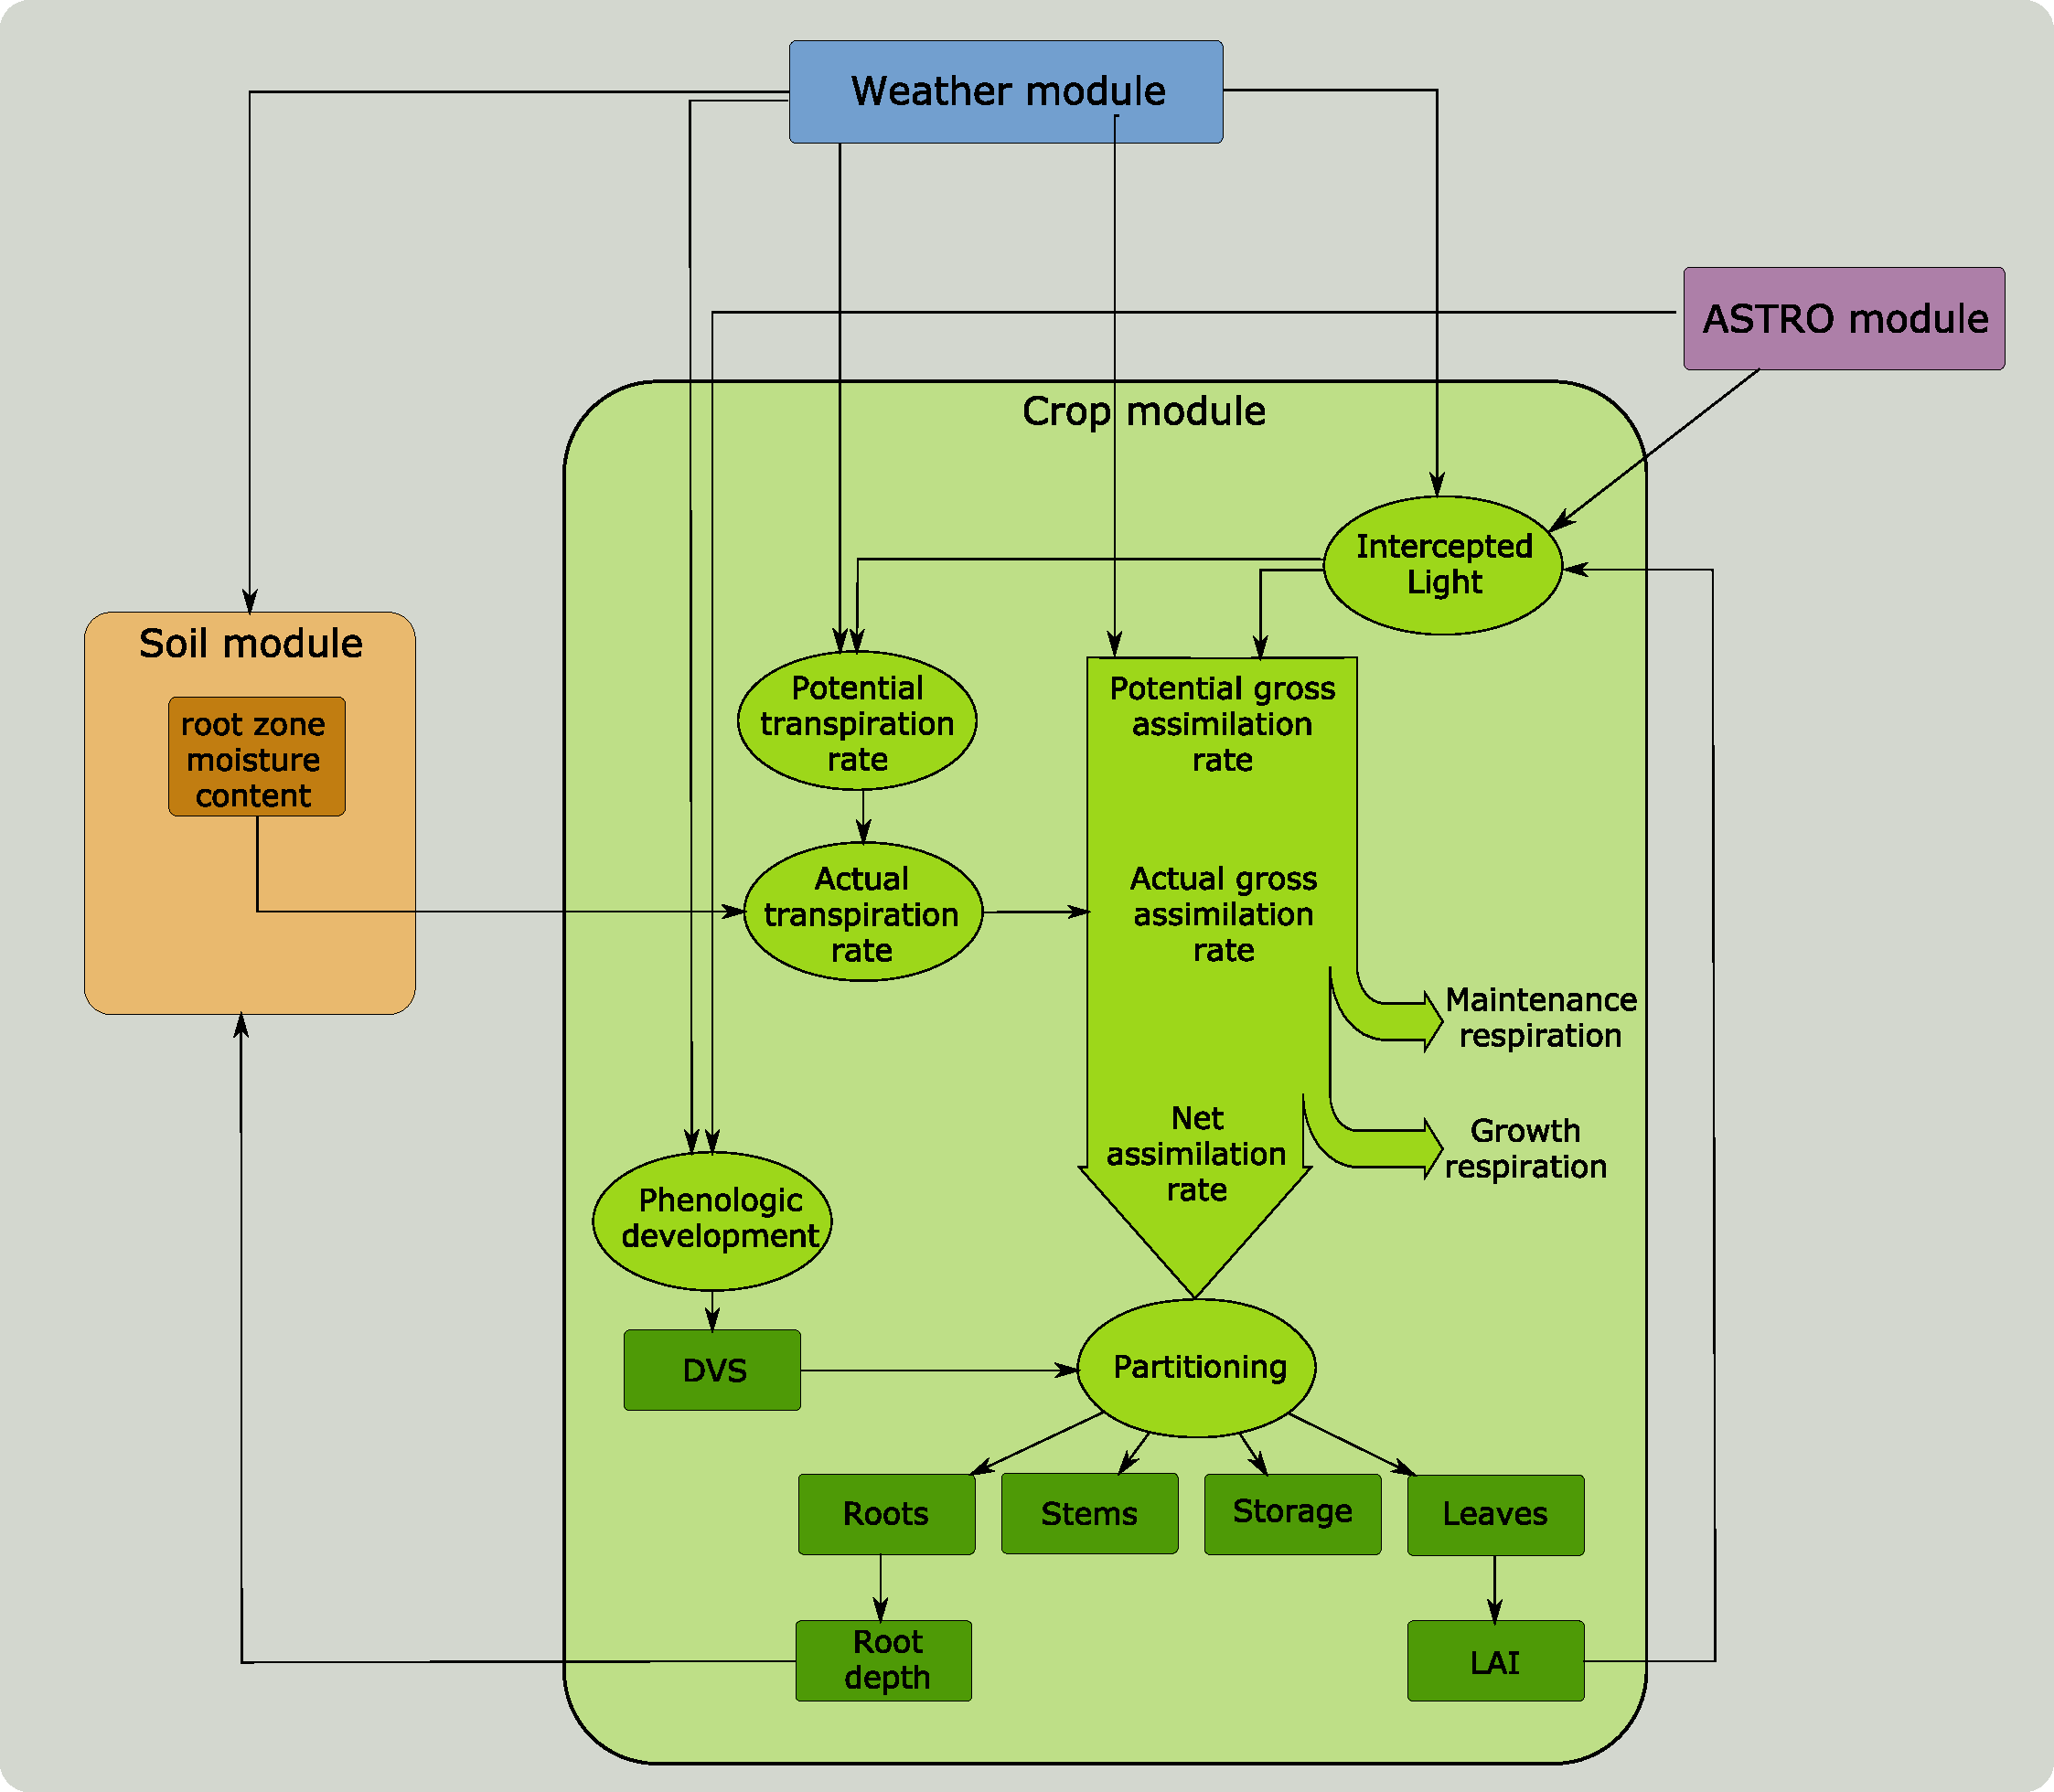
\includegraphics[width=\textwidth ]{\FigDir/wofost_schema_v3.pdf}
	\caption{Schematic overview of the major processes implemented in WOFOST and their linkages.}
	\label{fig:CropGrowthProc2}
\end{figure}

\section{Phenological development of a crop}

The physiological age of a plant is defined by the development stage (DVS), which on its turn is
characterized by the formation of the various organs and their appearance. The most
important phenological change is the one from vegetative to the reproductive stage, which
determines the most important change in the dry matter allocation over organs. As many
physiological and morphological processes change with the phenological stage of the
plant, accurate quantification of phenological development is essential in any simulation
model for crop growth. In WOFOST, the development stage is expressed in a dimensionless variable, 
having the value -0.1 at sowing, 0 at seedling emergence, 1 at flowering and 2 at maturity. 

In recent years the BBCH scale (https://en.wikipedia.org/wiki/BBCH-scale) was developed to provide 
a framework for defining phenological scales for a variety of crops. The phenological stages
used by WOFOST roughly correspond to BBCH scales 0 (sowing), 1 (leaf development), 6 (flowering)
and 9 (senescence). Converting the internal of WOFOST to use the BBCH scale for phenology is 
not trivial because many WOFOST parameters are defined as a function of DVS. Nevertheless,
in calibration studies it was demonstrated that specific DVS values can be linked consistently
to specific BBCH stages. Although the exact DVS values for a crop to reach a specific BBCH
stages can be variety specific.


\subsection{Crop emergence}

As start of the growing season the date of sowing or of emergence can be chosen. For a
photosynthesis-driven model like WOFOST, the simulation of crop growth starts at
emergence. If the sowing date is chosen by the model user, the day of emergence is
determined by the model. The crop emergence can be
defined as a function of the effective daily temperature sum since sowing date. Emergence
takes place when the effective daily temperature sum reaches the threshold temperature
for emergence (acronym: {\bf TSUMEM}). This threshold temperature is crop specific and
should be given by the user. The daily effective temperature depends on the base
temperature {\bf TBASEM}, below which no germination processes take place, and the maximum daily
temperature, beyond which the germination activity does not increase anymore {\bf TEFFMX}.
Both are crop specific. An example of this effective daily temperature as a function of daily
average temperature is depicted in figure \ref{fig:TEFFMAX}.

\begin{figure}[p]
	% fig 5.2
	\centering
	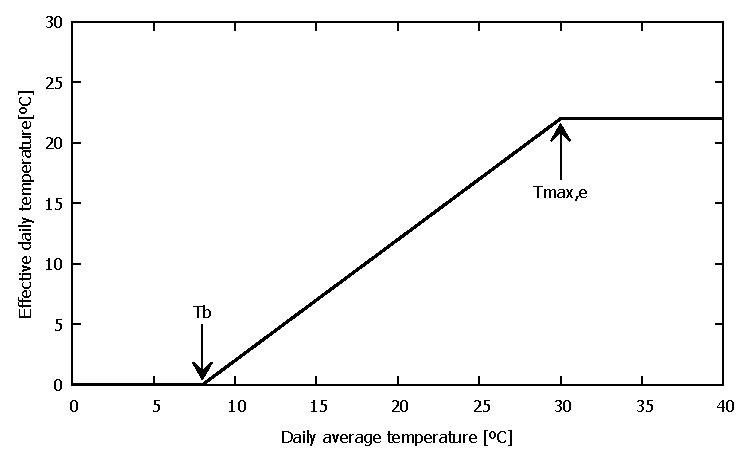
\includegraphics[width=120mm]{\FigDir/figure_TEFFMX.pdf}
	\caption{Effective temperature from sowing to emergence} 
	\label{fig:TEFFMAX}
\end{figure}

The following relationship can be defined for the effective temperature sum:

\begin{align}
T_{e} &= 0            & T \le T _{b} \nonumber  \\
T_{e} &= T~-~ T _{b}  & T _{b} ~<~T ~ < ~T _{\max ,e} \nonumber  \\
T_{e} &= T _{\max ,e} & T _{b} T \ge  T _{\max \, ,\, e}
\end{align}

Where:\\[5pt]
\begin{tabularx}{\textwidth}{llXr}
	T$_{{\rm e}}$ &:& Effective daily temperature & 
	[\degrees C]\\
	T$_{{\rm max,e}}$ &:& Maximum temperature beyond which phenological 
	activity does not increase    &    [\degrees C]\\
	T$_{{\rm b}}$ &:& Base temperature below which phenological development stops & 
	[\degrees C]\\
	T  &:& (Average) daily temperature & [\degrees C]
\end{tabularx}

Species originating from temperate regions show a base temperature of
0$-$3\degrees C, while species of subtropical and tropical origins have a base temperature of
9$-$14\degrees C (Angus {\it et al.}, 1981). Within a species, cultivars may vary substantially 
in their temperature requirements. The temperature sum, therefore, must be characterized for
each cultivar or group of cultivars (maturity classes).   

\subsection{Phenological development stage}
\label{sec:DVS}

A crop passes through successive phenological development stages. In WOFOST these stages 
are expressed in degree-days and defined by two parameters. The TSUM1 parameter defines
the number of degree-days for the emergence-anthesis period, while the TSUM2 parameter
defines the number of degree-days for the anthesis-maturity period. 
The length of these stages (in days) depends on the development rate. Development rates are 
controlled by vernalization requirements, day length and temperature. In the model before
anthesis, all factors can be active. After anthesis only temperature influence is possible.

Temperature is the main environmental factor affecting the development rate. Higher
temperatures increase the development rate leading to shorter growing periods. This rate
responds to temperature according to a curvilinear relationship. However, it has often
been demonstrated, that over a wide range of temperatures, the development rate
increases more or less linearly with temperature (van Dobben, 1962; van Keulen \&
Seligman, 1987).

In the model a flexible relation is used where the effective increase in temperature
sum, used for the calculation of the development rate, is dependent on the daily temperature 
(Summerfield \& Roberts, 1987). This relation is specified in an AFGEN table, 
allowing to account for non-linearity (lower and upper threshold values and optimum
ranges). The average temperature is the independent variable in the AFGEN table (see
Appendix 2). 

The development rate based on temperature can be reduced by the effect of vernalization and 
day length and can thus be obtained by:

\begin{equation}
% eq 5.3
\label{eq:5.3}
D_{r,t} = {f_{vern}}{f_{dayl}}{\frac{DT_{s}}{\sum T_{i}}}
\end{equation}

Where:\\[5pt]
\begin{tabularx}{\textwidth}{llXr}
	$f_{{\rm vern,t}}$ &:& Reduction factor for vernalization at time step t  & [-]\\
	$f_{{\rm dayl,t}}$ &:& Reduction factor for day length at time step t  & [-]\\
	D$_{{\rm r,t}}$ &:& Development rate at time step t  & [d$^{{\rm -1}}$]\\
	DT$_{{\rm s}}$ &:& Daily effective temperature & [\degrees C]\\
	$\sum$T$_{{\rm i}}$ &:& Temperature sum required to complete stage i & [\degrees C d]\\
\end{tabularx}

The temperature dependent correction factor, {\bf DT$_{{\rm s}}$} (acronym: {\bf DTSMTB}) and 
the temperature sum required to complete stage i, {\bf $\sum$T$_{{\rm i}}$} (acronym: 
{\bf TSUM1} or {\bf TSUM2}) are crop dependent and should be provided by the user.

The development stage at time step t is the integral of the development rate over the time
(i.e. time span from emergence to current time step) and can be calculated according to:

\begin{equation}
\label{eq:5.4}
D_{s,t} ~=~ D_{s,t-1} + D_{r,t} \Delta t
\end{equation}

Where:\\[5pt]
\begin{tabularx}{\textwidth}{llXr}
	D$_{{\rm s,t}}$ &:& Development stage at time step t    &    [-]\\
	D$_{{\rm r,t}}$ &:& Development rate at time step t     &   [d$^{{\rm -1}}$]\\
	$\Delta$t &:& Time step   &     [d]\\
\end{tabularx}

\subsection{Day length}

For certain crops or cultivars, during the vegetative stage (i.e. D$_{{\rm s}}$ $<$ 1), the 
effect of day length should be taken into account (e.g. "photosensitivity"). Moreover, crops 
that are sown in autumn
in temperate climate often require exposure to the prolonged cold of winter in order to be
able to flower. This effect is called the "vernalization requirement" of the crop.

Approaches that describe the effect of day length 
quantitatively are given amongst others by  Weir {\it et al.} (1984), Hadley {\it et al}. (1984) 
and Reinink {\it et al.} (1986). In WOFOST, a reduction factor for the development rate as a 
function of the day length is introduced. In case of photosensitivity can be calculated as:

\begin{equation}
\label{eq:5.5}
f_{red} ~=~{\frac{D ~-~D _{c} }{D _{o} ~-~ D _{c} }} ~~~~~~~~~0~\le ~f _{red} ~\le ~1
\end{equation}

Where:\\[5pt]
\begin{tabularx}{\textwidth}{llXr}
	$f_{{\rm dayl}}$ &:& Development rate reduction factor as function of day length   &     [-]\\
	D &:& Present day length (see eq. \ref{eq:AstroDaylength})   &     [h]\\
	D$_{{\rm c}}$ &:& Critical day length for development (lower threshold)    &    [h]\\
	D$_{{\rm o}}$ &:& Optimum day length for development (upper threshold)    &    [h]\\
\end{tabularx}

The user should provide information whether the development rate depends on temperature, 
on day length or on temperature and day length (acronym: {\bf IDSL}). The critical
daylength, {\bf D$_{{\rm c}}$} (acronym: {\bf DLC}) and the optimum daylength, 
{\bf D$_{{\rm o}}$} (acronym: {\bf DLO}) are crop dependent and should also be provided by 
the user. 

Note that in modern cultivars, photosensitivity is much less pronounced than in traditional
cultivars, and that for the purpose of modelling the day length influence can often be ignored.
However, for winter crops influence of day length and vernalization must be taken into
account in order to avoid that the choice of the sowing date in autumn has a large impact on 
the flowering and maturity date of the crop.


\subsection{Vernalization}

Vernalization is the induction of a plant's flowering process by exposure to the prolonged cold of winter, or by an artificial equivalent. After vernalization, plants have acquired the ability to flower, but they may require additional seasonal cues or weeks of growth before they will actually flower (source: Wikipedia). 

In WOFOST vernalization is simulated by assuming that a crop requires a number of (cultivar-specific)
vernalization days in order to reach its vernalization requirement. One vernalization day is added to the 
vernalization state 
when the daily average temperature is within the optimal temperature range for vernalization. A fractional
day or zero  is added when the temperature is outside of this range. This is rate of vernalization
(acronym: {\bf VERNR}) is decribed using an AFGEN table (acronym:  {\bf VERNRTB}) which describes the
temperature response curve for vernalization (figure \ref{fig:VERNRTB}).

The reduction factor on development rate is than derived by linearly scaling the current vernalization state 
((acronym:  {\bf VERN}))  between a base vernalization ((acronym:  {\bf VERNBASE})) and the number of 
days required to saturate the vernalization requirement (acronym:  {\bf VERNSAT}). The reduction 
factor can thus be expressed as: 

\begin{equation}
\label{eq:vern_factor}
f_{vern} ~=~{\frac{V ~-~V_{base} }{V _{sat} ~-~ V_{base} }} ~~~~~~~~~0~\le ~f _{vern} ~\le ~1
\end{equation}

Where:\\[5pt]
\begin{tabularx}{\textwidth}{llXr}
	$f_{{\rm vern}}$ &:& Development rate reduction factor as function of vernalization state   &     [-]\\
	$V$ &:& Present vernalization state of the crop   &     [days]\\
	$V_{{\rm base}}$ &:& Base vernalization for development (lower threshold)    &    [days]\\
	$V_{{\rm sat}}$ &:& Saturated vernalization for development (upper threshold)    &    [days]\\
\end{tabularx}

Note that it is possible for crops under certain conditions to de-vernalize, but this effect is not taken
into account in WOFOST.

\begin{figure}[p]
	% fig 5.2
	\centering
	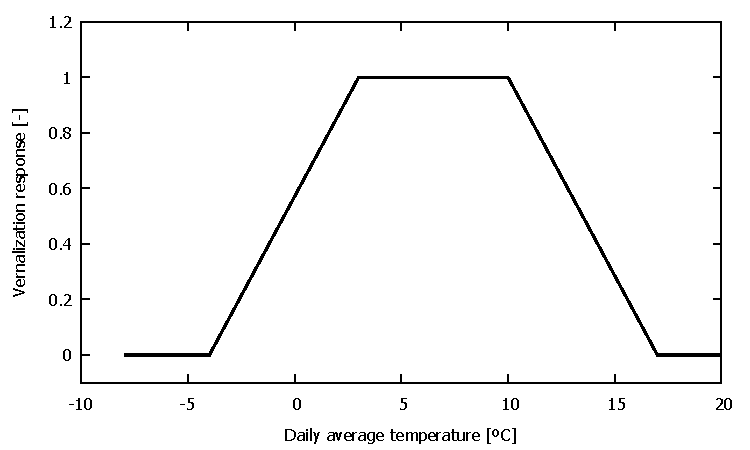
\includegraphics[width=120mm]{\FigDir/figure_VERNRTB.pdf}
	\caption{Response function for vernalization as a function
	of daily average temperature.} 
	\label{fig:VERNRTB}
\end{figure}

\subsection{End of the crop cycle}

The simulation of crop growth stops when the development stage reaches the stage at
which the crop will be harvested (acronym: {\bf DVSEND}). For crops that are harvested
at maturity {\bf DVSEND}) will be equal to 2.0. However, for crops that are deliberately
harvested earlier (e.g. silage maize) the value can be lower. For crops that are harvested
at a defined date, the value for {\bf DVSEND}) will be ignored.

\section{Daily assimilation} 

Daily dry matter production is the most detailed part of the model. The following steps
can be distinguished and will be described separately:
\begin{itemize}
	\item Total instantaneous gross CO$_{{\rm 2}}$ assimilation of the canopy 
	[\S \ref{sec:InstantGrossAssimilation}]
	\item Total daily gross CO2 assimilation rate of the canopy 
    [\S \ref{sec:DailyGrossAssimilation}]
	\item Actual daily gross photosynthesis rate of the canopy
	including temperature and development stage effect
    [\S \ref{sec:DailyGrossPhotosynthesis}]
	\item Reductions due to water and nutrient shortages
    [\S \ref{sec:evapotranspiration}]
\end{itemize}

The daily rate of CO$_{{\rm 2}}$ assimilation of the crop is driven by the intercepted light and can
be obtained by integrating the total instantaneous CO$_{{\rm 2}}$ assimilation rate of the canopy over
the day. The total instantaneous assimilation rate is calculated in subroutine {\bf ASSIM}, the
integration of the total instantaneous assimilation rate in subroutine {\bf TOTASS}. Both
calculations make use of the 3-point Gaussian integration method for calculating daily total 
gross assimilation (Goudriaan, 1986; Spitters, 1986).
Finally, actual gross photosynthesis is computed by applying correction factors for temperature,
water stress and nutrient stress onto the total daily assimilation

\subsection{Total daily gross CO$_{{\rm 2}}$ assimilation rate of the canopy}
\label{sec:DailyGrossAssimilation}

To calculate the total daily gross CO$_{{\rm 2}}$ assimilation rate of the whole canopy, an integration over time should be performed. Therefore, for given fluxes of photosynthetically
active radiation, at three different periods of the day, the total instantaneous gross canopy
CO$_{{\rm 2}}$ assimilation rate is computed. Afterwards, the integral of the total instantaneous
gross canopy CO$_{{\rm 2}}$ assimilation rate over time, as a weighted average of the selected three
hours, is calculated (Gaussian integration, see Appendix 1).

For the calculation of the total instantaneous gross canopy CO$_{{\rm 2}}$ assimilation rate, an
integration over depth of the gross instantaneous assimilation rate has to be performed.
Therefore, at three different depths in the canopy the gross instantaneous assimilation rate
is calculated, whereafter the integral of the gross instantaneous assimilation rate over
depth, as a weighted average of the selected depths, is computed (Gaussian integration,
see Appendix 1)

Integration, to calculate the daily total assimilation, is only necessary if instantaneous
assimilation will take place. Instantaneous assimilation will be zero if the leaf area index
equals zero (no photosynthetic activity). A second restriction for the integration is the
maximum CO$_{{\rm 2}}$ assimilation rate as a function of development stage, which is crop
dependent. When this maximum assimilation rate at light saturation equals zero also no
instantaneous assimilation will take place and no integration has to be performed.

As is mentioned before, in order to integrate the gross instantaneous assimilation rate
over the day, three points in time are selected to calculate the photosynthetically active
radiation. In this particular case, the radiation is homogeneously distributed over the day
according to the sine of the solar elevation, so the weighted average CO$_{{\rm 2}}$ 
assimilation rate can therefore be calculated for half a day only.

The three points in time are selected from noon to sunset (this explains the use of the
constants 0.5 and 12.00):

\begin{equation}
% eq 5.6
t_{h} = 12 + 0.5 \cdot D \cdot (0.5 ~+~ p\, \sqrt{0.15}) ~~~ for ~~~ p = -1,0,1
\end{equation}

Where:\\[5pt]
\begin{tabularx}{\textwidth}{llXr}
	D &:& Day length (see eq. \ref{eq:AstroDaylength})    &    [h]\\
	t$_{{\rm h}}$ &:& Hour of the day  &      [h]\\
	p &:& Gaussian integration points  &      [-]\\
\end{tabularx}

The incoming radiation and therefore gross assimilation rate, changes with solar elevation. 
The solar height as a function of the hour of the day can be calculated with:

\begin{equation}
\label{eq:5.7}
\sin \beta ~=~ \sin \lambda \, \sin \sigma ~+~ \cos \lambda \, \cos \sigma \, \cos \, 
(\, 2 \pi \,{\frac{t _{h} ~+~ 12}{24}} )
\end{equation}


Where:\\[5pt]
\begin{tabularx}{\textwidth}{llXr}
	$\beta$ &:& Solar elevation   &    [degrees]\\
	$\sigma$ &:& Solar declination    &    [degrees]\\
	$\lambda$ &:& Latitude     &   [degrees]\\
	t$_{{\rm h}}$ &:& Hour of the day    &    [h]\\
\end{tabularx}

Measured or estimated daily global solar radiation  (wavelength 300 - 3000 nm) is input
in the model. Only half of this incoming radiation is photosynthetically active (PAR,
Photosynthetically Active Radiation, wavelength 400 - 700 nm). This fraction, which is
generally called 'light' or 'visible radiation', is used in the calculation procedure of the
CO$_{{\rm 2}}$ assimilation rate of the canopy. In the model, the instantaneous incoming 
photosynthetically active radiation is calculated by multiplying half of the daily global radiation
with the ratio of the actual effective solar elevation and the integral of the effective solar
height (see also eq. \ref{eq:IntSolarHeight}):

\begin{equation}
\label{eq:5.8}
I _{0} ~=~ 0.5\, S _{g,d} \,{\frac{\sin \beta \, (\, 1~+~0.4\, \sin \beta \, )}{\int \, \sin \beta _{m} }}
\end{equation}

Where:\\[5pt]
\begin{tabularx}{\textwidth}{llXr}
	I$_{{\rm 0}}$ &:& Photosynthetically active radiation flux    &    
	[J m$^{{\rm -2}}$ s$^{{\rm -1}}$]\\
	S$_{{\rm g,d}}$ &:& Daily global radiation   &     
	[J m$^{{\rm -2}}$ d$^{{\rm -1}}$] \\
	$\beta$ &:& Solar elevation    &    [degrees]\\
	$\int \sin \beta_{{\rm m}}$ &:& The corrected integral of solar height over the day 
	for non homogeneous atmospheric transmission (eq. \ref{eq:IntSolarHeight})   
	&     [s]\\
\end{tabularx}

The calculated photosynthetically active radiation flux consists of a diffuse flux and a
direct flux. The diffuse flux is the result of scattering of sun rays by clouds, aerosols and
gases in the atmosphere. The proportion of diffuse light in the total incident light flux
depends on the status of the atmosphere (see also eq. \ref{eq:irrad_diffuse}). This fraction 
is calculated from the atmospheric transmission using an empirical function (Spitters 
{\it et al.}, 1986).

\begin{equation}
% eq 5.9
I_{0,df} ~=~ D _{p~} \sin \beta
\end{equation}

Where:\\[5pt]
\begin{tabularx}{\textwidth}{llXr}
	I$_{{\rm 0,df}}$ &:& Diffuse part of the photosynthetically active radiation flux 
	at top of the canopy    &    [J m$^{{\rm -2}}$ s$^{{\rm -1}}$]\\
	D$_{{\rm p}}$ &:& Diffuse radiation perpendicular to the direction 
	light (see eq. 4.31)    &    [J m$^{{\rm -2}}$ s$^{{\rm -1}}$]\\
	sin$\beta$ &:& Solar elevation (see eq. \ref{eq:5.7})    &    [degrees]\\
\end{tabularx}

The direct part can be easily obtained by subtracting the diffuse part from the
photosynthetically radiation flux:

\begin{equation}
% eq 5.10
I_{0,dr} ~=~ I_{0} ~-~I_{0,df} 
\end{equation}

Where:\\[5pt]
\begin{tabularx}{\textwidth}{llXr}
	I$_{{\rm 0,dr}}$ &:& Direct part of the photosynthetically active radiation flux 
	at top of the canopy    &    [J m$^{{\rm -2}}$ s$^{{\rm -1}}$]\\
	I$_{{\rm 0}}$ &:& Photosynthetically active radiation flux (see eq. \ref{eq:5.8})    &  
	[J m$^{{\rm -2}}$ s$^{{\rm -1}}$]\\
	I$_{{\rm 0,df}}$ &:& Diffuse part of the photosynthetically active radiation flux 
	at top of the canopy     &   [J m$^{{\rm -2}}$ s$^{{\rm -1}}$]\\
\end{tabularx}

Once the photosynthetically active radiation fluxes have been established, the 
instantaneous gross assimilation rate of the canopy can be calculated (see \S
\ref{sec:InstantGrossAssimilation}). And the integration over time can take place.
The integral of the total gross canopy assimilation rate over time is calculated as the
weighted average of the three selected hours of the day. Multiplying by the day length
results in the total daily gross rate of CO$_{{\rm 2}}$ assimilation. 

\begin{equation}
\label{eq:5.11}
A_{d} = D {\frac{A_{C,-1} ~+~ 1.6 A_{C,0} ~+~ A_{C,1} }{3.6}}
\end{equation}

Where:\\[5pt]
\begin{tabularx}{\textwidth}{llXr}
	A$_{{\rm d}}$ &:& Total gross assimilation rate    &    
	[kg ha$^{{\rm -1}}$ d$^{{\rm -1}}$]\\
	D &:& Day length (see eq. \ref{eq:AstroDaylength})   &     [h]\\
	A$_{{\rm C}}$ &:& Total inst. gross assimilation rate for
	the whole canopy, p= -1,0,1 (see eq. \ref{eq:5.31})    &
	[kg ha$^{{\rm -1}}$ h$^{{\rm -1}}$]\\
\end{tabularx}

\subsection{Total instantaneous gross CO$_{2}$ assimilation of the canopy}  
\label{sec:InstantGrossAssimilation}

In the subroutine {\bf ASSIM}, the total instantaneous rate of CO$_{{\rm 2}}$ assimilation of the canopy is
calculated from the incoming fluxes of diffuse and direct photosynthetic active radiation,
solar elevation and leaf area index and several parameters.

\subsubsection{Reflection and extinction}
The total incoming photosynthetically active radiation flux is partly reflected by the
canopy. The reflection coefficient is defined as the fraction of the downward radiation
flux that is reflected by the whole canopy. According to Goudriaan (1977), the reflection
coefficient of a green leaf canopy with a random spherical leaf angle equals:

\begin{equation}
\label{eq:5.12}
\rho = {\frac{1- \sqrt{1-\sigma}}{1 + \sqrt{1-\sigma}}} \cdot {\frac{2}{1+1.6 \sin \beta }}
\end{equation}

Where:\\[5pt]
\begin{tabularx}{\textwidth}{llXr}
	$\rho$ &:& Reflection coefficient of a green leaf canopy    &    [-]\\
	$\sigma$ &:& Scattering coefficient fraction (transmission and reflection) 
	of single leaves for visible radiation   
	{\small (=0.2; Goudriaan, cited by Spitters, 1986)}  &     [-]\\  
	$\beta$ &:& Solar elevation (see eq. \ref{eq:SolarElevation})    &    [degrees]\\
\end{tabularx}

The first term denotes the reflection of the canopy of horizontal leaves and the second
term is the approximate correction factor for a spherical leaf angle distribution.

A fraction (1-$\rho$) of the incoming visible radiation is potentially available for absorption by
the canopy. Radiation fluxes attenuate exponentially within a canopy with increasing leaf
area from the top downwards:

\begin{equation}
\label{eq:5.13}
I_{L~} = I_{0} (1~-~\rho ) e^{-\kappa LAI_{L} }
\end{equation}

Where:\\[5pt]
\begin{tabularx}{\textwidth}{llXr}
	I$_{{\rm L}}$   &:& Net photosynthetic active radiation flux at 
	depth L in the canopy    &    [J m$^{{\rm -2}}$ s$^{{\rm -1}}$]\\
	I$_{{\rm 0}}$   &:& Photosynthetically active radiation flux (see eq. \ref{eq:5.8})  & 
	[J m$^{{\rm -2}}$ s$^{{\rm -1}}$]\\
	LAI$_{{\rm L}}$ &:& Cumulative leaf area index (from top downwards) 
	relative depth L & [ha ha$^{{\rm -1}}$]\\
	$\rho$          &:& Reflection coefficient of the canopy   &     [-]\\
	$\kappa$        &:& Extinction coefficient for photosynthetic active 
	radiation flux   &     [-]\\
\end{tabularx}

The diffuse and the direct flux have different extinction coefficients, giving rise to
different light profiles within the canopy for diffuse and direct radiation. Therefore three
different radiation fluxes are distinguished:
\begin{itemize}
	\item the diffuse flux, with extinction coefficient $\kappa_{df}$;
	\item the total direct flux, with extinction coefficient $\kappa_{dr,t}$;
	\item the direct component of direct light, with extinction coefficient $\kappa_{dr,bl}$.
\end{itemize}

Radiation becomes diffuse when sun rays are partly absorbed and partly scattered (i.e.
reflected or transmitted) by a leaf. The subscript {\it bl} (black) is used, the leaves show
neither transmission nor reflection. The extinction coefficient of 'black leaves'
can be calculated as:

\begin{equation}
% eq 5.14
\label{eq:5.14}
\kappa_{bl} ~=~{\frac{0.5}{\sin \beta }}
\end{equation}

Where:\\[5pt]
\begin{tabularx}{\textwidth}{llXr}
	$\kappa$$_{{\rm bl}}$ &:& Extinction coefficient for the direct radiation flux   &     [-]\\
	$\beta$ &:& Solar elevation    &    [degree]\\
\end{tabularx}

For a spherical leaf area distribution (homogeneous, random), the extinction coefficient
for the diffuse radiation flux equals:

\begin{equation}
\label{eq:5.15}
\kappa_{df} ~=~ \kappa_{bl} \, \sqrt{1~-~ \sigma }
\end{equation}

Where:\\[5pt]
\begin{tabularx}{\textwidth}{llXr}
	$\kappa$$_{{\rm df}}$ &:& Extinction coefficient for the diffuse radiation flux    &    [-]\\
	$\sigma$ &:& Scattering coefficient fraction of single leaves for 
	visible radiation    &    [-]\\
\end{tabularx}

In the model, the extinction coefficient for the diffuse radiation flux, 
{\bf $\kappa$$_{{\rm df}}$} (acronym: {\bf KDIF})
is not computed but should be provided by the user. It can be measured directly 
under diffuse sky conditions.

In equation \ref{eq:5.14}, 0.5 points to the average projection on the ground surface of leaves
showing a spherical angle distribution, and 0.8 in equation \ref{eq:5.16} is the value of 0.5/sin$\beta$
averaged over elevation $\beta$ of incident radiation under an overcast sky.

The average extinction coefficient for the diffuse radiation flux is about 0.72 (Goudriaan,
1977). However, in many situations, the leaf angle distribution is not spherical. For
example in rice, the leaves are clustered (especially in the beginning as a result of
planting on hills), and have a very vertical orientation. Other leaf angle distributions can
be accounted for by a procedure described by Goudriaan (1986), which calculates the
extinction coefficient for the diffuse radiation flux on the basis of the frequency 
distribution of leaves with angles in different classes.

In the model however, the leaf angle distribution is accounted for by using a so called
cluster factor which is the measured extinction coefficient for diffuse radiation flux,
relative to the theoretical one for a spherical leaf area distribution. The cluster factor can
be calculated as: 

\begin{equation}
\label{eq:5.16}
C _{f} ~=~{\frac{ \kappa _{df} }{0.8\, \sqrt{1 ~-~ \sigma } }}
\end{equation}

Where:\\[5pt]
\begin{tabularx}{\textwidth}{llXr}
	C$_{{\rm f}}$ &:& Cluster factor    &    [-]\\
	$\kappa$$_{{\rm df}}$ &:& Extinction coefficient for diffuse radiation flux   &     [-]\\
	$\sigma$ &:& Scattering coefficient fraction of single leaves for
	visible radiation  &      [-]\\
\end{tabularx}

The direct component can be calculated as (Goudriaan, 1977):

\begin{equation}
\label{eq:5.17}
\kappa _{dr,bl} ~=~{ C _{f} }\,{\frac{0.5}{\sin \beta }}
\end{equation}

Where:\\[5pt]
\begin{tabularx}{\textwidth}{llXr}
	$\kappa$$_{{\rm dr,bl}}$ &:& Extinction coefficient for the direct component of direct light   &     [-] \\
	C$_{{\rm f}}$ &:& Cluster factor     &   [-]\\
	$\beta$ &:& Solar elevation     &   [degrees]\\
\end{tabularx}

The extinction coefficient for the total direct radiation flux can be calculated as (Goudriaan, 1977):

\begin{equation}
\label{eq:5.18}
\kappa _{dr,t} ~=~ \kappa _{dr,bl} \sqrt{1~-~\sigma }
\end{equation}

Where:\\[5pt]
\begin{tabularx}{\textwidth}{llXr}
	$\kappa_{dr,t}$ &:& Extinction coefficient for total direct radiation flux   &    [-]\\
	$\kappa_{dr,bl}$ &:& Extinction coefficient for the direct component of direct light  &   [-]\\
	$\sigma$ &:& Scattering coefficient     &    [-]\\
\end{tabularx}

\subsubsection{Absorption}
Three depths in the canopy are selected according to the Gaussian integration method (see
Appendix 1) and at those levels the leaf area index, the amount of absorbed radiation and
the leaf CO$_{{\rm 2}}$ assimilation is calculated. The total instantaneous assimilation is easily
obtained by multiplying the instantaneous assimilation with the total leaf area index (eq.
\ref{eq:5.31}). In the following text the calculation processes, concerning the instantaneous
assimilation, will be explained in detail. Calculation of the leaf area index will be
explained in \S \ref{sec:growthofleaves}.

Canopy assimilation is calculated as a weighted average of the assimilation at three
horizons within the canopy. The leaf area index of the selected horizons can be written as
(Goudriaan, 1986):

\begin{equation}
% eq 5.19 a-d
LAI_{L} = (0.5 + p \sqrt{0.15}) \cdot LAI~~~~for~~~~p = -1,0,1
\end{equation}


Where:\\[5pt]
\begin{tabularx}{\textwidth}{llXr}
	LAI$_{{\rm L}}$ &:& Leaf area index at relative distance L in the canopy 
	(L=0 at the top)    &    [ha ha$^{{\rm -1}}$]\\
\end{tabularx}

The light absorbed at a certain depth in the canopy is obtained by taking the derivative of
equation \ref{eq:5.13} with respect to the cumulative leaf area index:

\begin{equation}
% eq 5.20
I_{a,L} = {\frac{-dI _{0\, ,\, L} }{dL}} = \kappa (1 -  \rho) I_{0} \cdot e^{- \kappa LAI_{L}}
\end{equation}

Where:\\[5pt]
\begin{tabularx}{\textwidth}{llXr}
	I$_{{\rm a,L}}$ &:& Amount absorbed of total radiation flux
	\footnote{With the 'Total radiation flux' in this paragraph the total photosynthetically 
		active radiation flux is meant.} at relative depth L    &    
	[J m$^{{\rm -2}}$ s$^{{\rm -1}}$]\\
	I$_{{\rm 0,L}}$ &:& Net photosynthetic active radiation at relative depth L in 
	the canopy    &    [J m$^{{\rm -2}}$ s$^{{\rm -1}}$]\\
	I$_{{\rm 0}}$ &:& Photosynthetically active radiation flux at top of the 
	canopy   &     [J m$^{{\rm -2}}$ s$^{{\rm -1}}$]\\
	L &:& Relative depth in the canopy   &     [-]\\
	$\kappa$ &:& The extinction coefficient for the PAR flux    &     [-]\\
	$\rho$ &:& Reflection coefficient of the canopy (see eq. \ref{eq:5.12})   &     [-]\\
\end{tabularx}

If expressed for the different light components, the absorbed fluxes for the different
components per unit leaf area at a certain depth in the canopy are:

\stepcounter{equation}
\begin{align}
% equation 5.21a-c
I_{a,df} &={\frac{-dI_{df,L}}{dL}} &
&= \kappa_{df} (1 - \rho)\, I_{0,df} \cdot e^{-\kappa_{df} \, LAI_{L}} \subeqn  \\
I_{a,dr,t} &= {\frac{-dI_{dr,t,L}}{dL}} & 
&= \kappa_{dr,t} (1-\rho) I_{0,dr} \cdot e^{-\kappa_{dr,t} LAI_{L}} \subeqn  \\
% TODO: check if below I_{a,dr,dr} should be changed to I_{a,dr,bl}
I_{a,dr,dr} &= {\frac{-dI_{dr,L}}{dL}} &
&= \kappa_{dr,bl} (1-\sigma) I_{0,dr} \cdot e^{-\kappa_{dr,bl} LAI_{L}} \subeqn
\end{align}

Where:\\[5pt]
\begin{tabularx}{\textwidth}{llXr}
	I$_{{\rm a,.}}$ &:& Amount absorbed of specified radiation flux   &      
	[J m$^{{\rm -2}}$ s$^{{\rm -1}}$]\\
	I$_{{\rm .,L}}$ &:& Net specified component of PAR flux at relative depth L    &    
	[J m$^{{\rm -2}}$ s$^{{\rm -1}}$]\\
	I$_{{\rm 0}}$ &:& Photosynthetically active radiation flux at top of the canopy
	(see eq. \ref{eq:5.8})   &   [J m$^{{\rm -2}}$ s$^{{\rm -1}}$]\\
	L &:& Relative depth in the canopy   &     [-]\\
	$\kappa$$_{{\rm .}}$ &:& The extinction coefficient for specified radiation 
	(see eq. \ref{eq:5.15}, \ref{eq:5.17} and \ref{eq:5.18})    &    [-]\\
	$\rho$ &:& Reflection coefficient of the canopy (see eq. \ref{eq:5.12})   &     [-]\\
	$\sigma$ &:& Scattering coefficient    &    [-]\\
	bl &:& Black &\\
	df &:& Diffuse &\\
	dr &:& Direct &\\
	t &:& Total &\\
\end{tabularx}

Note that of the direct component of the direct flux the non-scattered part (1-$\sigma$) is
absorbed.

The total absorbed flux for shaded leaves can be calculated as the sum of the absorbed
flux of diffuse radiation and absorbed flux of the diffuse radiation of the indirect
component of direct radiation. The last one is equal to the difference of the absorbed flux
of the total radiation minus the absorbed flux of the direct component of the direct
radiation.

\begin{equation}
\label{eq:5.22}
I _{a,sh} ~=~ I _{a,df} ~+~ (I_{a,dr,t} ~-~ I_{a,dr,dr} )
\end{equation}

Where:\\[5pt]
\begin{tabularx}{\textwidth}{llXr}
	I$_{{\rm a,sh}}$ &:& Absorbed amount of the total radiation flux by shaded leaves
	&    [J m$^{{\rm -2}}$ s$^{{\rm -1}}$]\\
	I$_{{\rm a,df}}$ &:& Absorbed amount of the diffuse radiation flux
	&     [J m$^{{\rm -2}}$ s$^{{\rm -1}}$]\\
	I$_{{\rm a,dr,t}}$ &:& Absorbed amount of the total direct radiation flux
	&     [J m$^{{\rm -2}}$ s$^{{\rm -1}}$]\\
	I$_{{\rm a,dr,dr}}$ &:& Absorbed amount of direct component of the  direct radiation flux
	& [J m$^{{\rm -2}}$ s$^{{\rm -1}}$]\\
\end{tabularx}


\subsubsection{Instantaneous gross assimilation}
The CO$_{{\rm 2}}$ assimilation-light response can be obtained by introducing the absorbed amount
of light into an assimilation-light response function of individual leaves. This assimilation-light
response curve is computed using an exponential function that requires the instantaneous assimilation 
rate at light saturation and the initial angle to be defined:

\begin{equation}
\label{eq:5.23}
A_{L} = A_{m} (1-\exp({{-\epsilon I_{a}}/{A_{m}}}))
\end{equation}

Where:\\[5pt]
\begin{tabularx}{\textwidth}{llXr}
	A$_{{\rm L}}$ &:& Inst.\footnote{ Inst. = Instantaneous} gross assimilation 
	rate at relative depth L (per unit leaf area)    &    
	[kg ha$^{{\rm -1}}$ h$^{{\rm -1}}$]\\
	A$_{{\rm m}}$ &:& Inst. gross assimilation rate at light saturation    & 
	[kg ha$^{{\rm -1}}$ h$^{{\rm -1}}$]\\
	$\epsilon$ &:& Initial light use efficiency   &   [(kg ha$^{{\rm -1}}$ 
	h$^{{\rm -1}}$)/(J m$^{{\rm -2}}$ s$^{{\rm -1}}$])\\
	I$_{{\rm a}}$ &:& Absorbed amount of the total radiation flux     &   
\end{tabularx}

The instantaneous gross assimilation rate at light saturation, {\bf A$_{{\rm m}}$} (acronym: {\bf AMAXTB}) is
crop specific. It is a function of the crop development stage and corrected for the ambient CO$_{2}$ 
concentration (acronym: {\bf CO2AMAXTB}). The initial light use efficiency, {\bf $\epsilon$}
(acronym: {\bf EFFTB}), is also crop dependent. It is defined as a function of daily mean temperature and
corrected for ambient CO2 concentration ((acronym: {\bf CO2EFFTB})). 

Introducing the absorbed amount of radiation by shaded leaves (eq. \ref{eq:5.22}) into 
equation \ref{eq:5.23} yields:

\begin{equation}
\label{eq:5.24}
A_{sh} = A_{m} \big(1-\exp({{-\epsilon I_{a,sh} }/{A_m}} ) \big)
\end{equation}

Where:\\[5pt]
\begin{tabularx}{\textwidth}{llXr}
	A$_{{\rm sh}}$ &:& Inst. gross assimilation rate for shaded leaves  & 
	[kg ha$^{{\rm -1}}$ h$^{{\rm -1}}$]\\
	A$_{{\rm m}}$ &:& Inst. gross assimilation rate at light saturation & 
	[kg ha$^{{\rm -1}}$ h$^{{\rm -1}}$]\\
	$\epsilon$ &:& Initial light use efficiency  &  
	[(kg ha$^{{\rm -1}}$ h$^{{\rm -1}}$)/(J m$^{{\rm -2}}$ s$^{{\rm -1}}$)]\\
	I$_{{\rm a,sh}}$ &:& Absorbed amount of the total radiation flux  by shaded leaves (see eq. \ref{eq:5.22})   &
	[J m$^{{\rm -2}}$ s$^{{\rm -1}}$]\\
\end{tabularx}

For the sunlit leaf area, the average absorption intensity may be substituted in equation
\ref{eq:5.23}. However, it is more accurate to account for the variation in leaf angle and thus in
illumination intensity (Spitters, 1986). The direct flux is absorbed by a leaf perpendicular
to the direct beam with an intensity of: 

\begin{equation}
\label{eq:5.25}
I_{a,dr,sl} = {\frac{(1-\sigma) I_{0,dr}}{\sin \beta }}
\end{equation}

Where:\\[5pt]
\begin{tabularx}{\textwidth}{llXr}
	I$_{{\rm a,dr,sl}}$ &:& Absorbed amount of the direct radiation flux by leaves
	perpendicular to the direct beam    &    [J m$^{{\rm -2}}$ s$^{{\rm -1}}$]\\
	I$_{{\rm 0,dr}}$ &:& Direct flux of visible radiation at the top of 
	the canopy &  [J m$^{{\rm -2}}$ s$^{{\rm -1}}$]\\
	$\sigma$ &:& Scattering coefficient  &[-]\\
	$\beta$ &:& Solar elevation   & [degrees]\\
\end{tabularx}

The amount of absorbed direct radiation by leaves (eq. \ref{eq:5.25}) depends on the sine of
incidence at the leaf surfaces. Therefore, for sunlit leaves, CO$_{{\rm 2}}$ assimilation rates have to
be calculated separately for leaves with different angles and integrated over the sine of
incidence. In the model a spherical leaf angle distribution is assumed, so no integration
over leaf angles is needed.

Integration over the sine of incidence for the sunlit leaves yields (Goudriaan, personal
communication):

\begin{equation}
% eq 5.26
A_{sl} = A_{m} \bigg( 
1-(A_{m} - A_{sh})  {\frac{1~- \exp({{-I _{a,dr,sl} \, \epsilon}}/{A_m}) }
	{\epsilon\, I _{a,dr,sl} }}
\bigg)
\end{equation}

Where:\\[5pt]
\begin{tabularx}{\textwidth}{llXr}
	A$_{{\rm sl}}$ &:& Inst. gross assimilation rate for sunlit leaves  &
	[kg ha$^{{\rm -1}}$ h$^{{\rm -1}}$]\\
	A$_{{\rm sh}}$ &:& Inst. gross assimilation rate for shaded leaves  &
	[kg ha$^{{\rm -1}}$ h$^{{\rm -1}}$]\\
	A$_{{\rm m}}$ &:& Inst. gross assimilation rate at light saturation &
	[kg ha$^{{\rm -1}}$ h$^{{\rm -1}}$]\\
	I$_{{\rm a,dr,sl}}$ &:& Absorbed amount of the direct radiation flux by leaves
	perpendicular to the direct beam  &  [J m$^{{\rm -2}}$ s$^{{\rm -1}}$]\\
	$\epsilon$ &:& Initial light use efficiency  &   [(kg ha$^{{\rm -1}}$ 
	h$^{{\rm -1}}$)/(J m$^{{\rm -2}}$ s$^{{\rm -1}}$)]\\
\end{tabularx}

The assimilation rate per unit leaf area at a specific depth in the canopy is the sum of the
assimilation rates of sunlit and shaded leaves, taking into account the proportion of sunlit
and shaded leaf area at that depth in the canopy. 

The fraction sunlit leaf area equals the fraction of the direct radiation reaching that layer:

\begin{equation}
% eq 5.27
f_{sl} =  e^{-\kappa_{dr,bl} \cdot LAI_{L}}
\end{equation}

Where:\\[5pt]
\begin{tabularx}{\textwidth}{llXr}
	f$_{{\rm sl}}$ &:& Fraction sunlit leaf area   &     [-]\\
	$\kappa$$_{{\rm dr,bl}}$ &:& Extinction coefficient for the direct component of
	direct radiation (see eq. \ref{eq:5.17})   &     [-]\\
	LAI$_{{\rm L}}$ &:& Cumulative leaf area index at relative depth L in canopy  &      [-]
\end{tabularx}

The total instantaneous assimilation rate at a relative depth L can be calculated as:

\begin{equation}
\label{eq:5.28}
A_{T,L} = f_{sl} A_{sl} + (1 - f_{sl}) A_{sh} 
\end{equation}

Where:\\[5pt]
\begin{tabularx}{\textwidth}{llXr}
	A$_{{\rm T,L}}$ &:& Total inst. gross assimilation rate at a relative depth L   &
	[kg ha$^{{\rm -1}}$ h$^{{\rm -1}}$]\\
	A$_{{\rm sl}}$ &:& Inst. gross assimilation rate for sunlit leaves  & 
	[kg ha$^{{\rm -1}}$ h$^{{\rm -1}}$]\\
	A$_{{\rm sh}}$ &:& Inst. gross assimilation rate for shaded leaves  & 
	[kg ha$^{{\rm -1}}$ h$^{{\rm -1}}$]\\
	f$_{{\rm sl}}$ &:& Fraction sunlit leaf area  &  [-]\\
\end{tabularx}

The total instantaneous assimilation rate for the whole canopy per unit leaf area can be
established using the Gaussian integration method, as a weighted average of the assimilation 
at three levels within the canopy.
However, first the leaf area index of the levels selected have to be established:

\begin{equation}
\label{eq:5.29}
LAI_{L} = (0.5+p \sqrt{0.15})LAI~~~~for~~~~p=-1,0,1
\end{equation}

Where:\\[5pt]
\begin{tabularx}{\textwidth}{llXr}
	LAI$_{{\rm L}}$ &:& Leaf area index at relative depth L in canopy    &    [ha ha$^{{\rm -1}}$]\\
	LAI &:& Total leaf area of the crop (see \S \ref{sec:growthofleaves}) &   [ha ha$^{{\rm -1}}$]\\
\end{tabularx}

Introducing the values of the leaf area index of the three selected layers in the equations
mentioned before, will yield the instantaneous assimilation at these horizons. The
weighted average of these values yields the total instantaneous assimilation rate for the
whole canopy per unit leaf area.

The weighted average of the total instantaneous assimilation rates can be calculated as:

\begin{equation}
% eq 5.30
A_{C,l} = {\frac{(A_{T,L,-1} + 1.6 A_{T,L,0} + A_{T,L,1})}{3.6}}
\end{equation}

Where:\\[5pt]
\begin{tabularx}{\textwidth}{llXr}
	A$_{{\rm C,l}}$ &:& Total instantaneous canopy assimilation 
	rate (per unit leaf area)    &    [kg ha$^{{\rm -1}}$ h$^{{\rm -1}}$]\\
	A$_{{\rm T,L,p}}$ &:& Total instantaneous gross assimilation rate at relative 
	depth L (see eq. \ref{eq:5.28}) at p= -1,0,1 (see eq. \ref{eq:5.29})    &    
	[kg ha$^{{\rm -1}}$ h$^{{\rm -1}}$]\\
\end{tabularx}

This total instantaneous assimilation rate is calculated per unit leaf area and must
therefore be multiplied with the leaf area index to yield the total assimilation rate for the
whole canopy:

\begin{equation}
\label{eq:5.31}
A_{C} = A_{C,l} \cdot LAI
\end{equation}

Where:\\[5pt]
\begin{tabularx}{\textwidth}{llXr}
	A$_{{\rm C}}$ &:& Total inst. gross assimilation rate for
	the whole canopy  &  [kg ha$^{{\rm -1}}$ h$^{{\rm -1}}$]\\
	A$_{{\rm C,l}}$ &:& Total inst. gross canopy assimilation rate 
	per unit leaf area &  [kg ha$^{{\rm -1}}$ h$^{{\rm -1}}$]\\
	LAI &:& Total leaf area of the crop (see \S \ref{sec:growthofleaves})  & [ha ha$^{{\rm -1}}$]\\
\end{tabularx}

Note that the green parts of the stems and the storage organs (like panicles) may absorb a
substantial amount of radiation. Therefore, the green area index of these organs is added
to the total leaf area. The green area index of the stems and storage organs can be
calculated by multiplying the dry weight of the organ with respectively the specific stem
area and the specific pod area (see also \S \ref{sec:growthofleaves} and eq. \ref{eq:5.24}). The specific 
stem area and specific pod area are crop specific and should be provided by the user.


\subsection{Reduction factor for daily gross assimilation rate}
\label{sec:DailyGrossPhotosynthesis}

In the previous section, the assimilation was treated as a function of the intercepted light and of
photosynthetic crop characteristics such as initial light use efficiency and maximum leaf
CO$_{{\rm 2}}$ assimilation at light saturation. The value of some crop characteristics are dependent
on phenological crop stage. In addition, the assimilation process can be hampered by
suboptimum temperatures and/or by reduced availability of CO$_{{\rm 2}}$ due to closure of the leaf
stomata as means to reduce transpiration. Finally, also nutrient deficiency can cause a reduction
in the assimilation rate.

Thus, the gross assimilation rate depends on development stage, on temperature, on the transpiration rate
and on plant nutrient status. In this paragraph this dependency will be briefly explained.

\subsubsection{Development stage}
As mentioned before, the instantaneous gross assimilation rate at light saturation, also
called the maximum leaf CO$_{{\rm 2}}$ assimilation rate, {\bf A$_{{\rm m}}$} (acronym: 
{\bf AMAXTB}) is a function of
the development stage and is crop specific. An AFGEN table with the development stage
as the independent variable is used to describe this dependency (see also \S \ref{sec:DVS}). For an
example see figure \ref{fig:AMAXTB}.

\begin{figure}[p]
	% figure 5.3
	\centering
	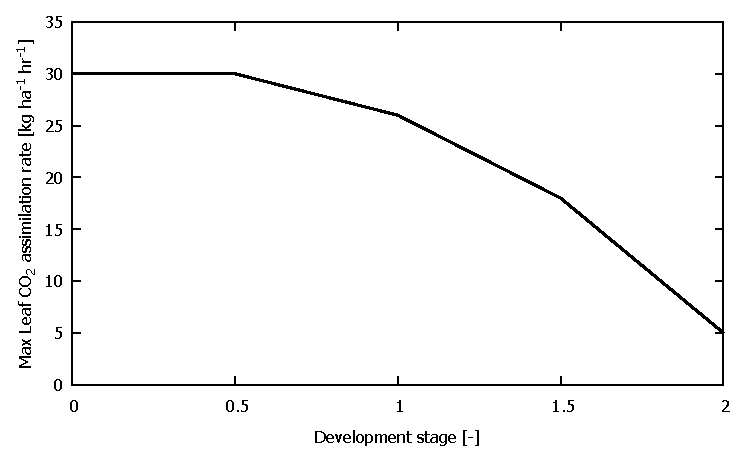
\includegraphics[width=85mm]{\FigDir/figure_AMAXTB.pdf}
	\caption{Maximum leaf CO$_{{\rm 2}}$ assimilation the rate as a function of development of
		the development stage.}
	\label{fig:AMAXTB}
\end{figure}

\subsubsection{Daytime temperature}
The maximum leaf CO$_{{\rm 2}}$ assimilation rate, A$_{{\rm m}}$, has to be corrected for sub-optimal average
daytime temperatures. The correction factor is determined by the average daytime
temperature and is also crop specific. An AFGEN table (acronym: {\bf TMPFTB}) with the
average day time temperature (\ref{eq:daytimetemp}) as the independent variable is used to describe this
dependency (see also Appendix 2). For an example see figure \ref{fig:TMPFTB}. 
The correction factor has to be multiplied with A$_{{\rm m}}$. 

\begin{figure}[p]
	%figure 5.4
	\centering
	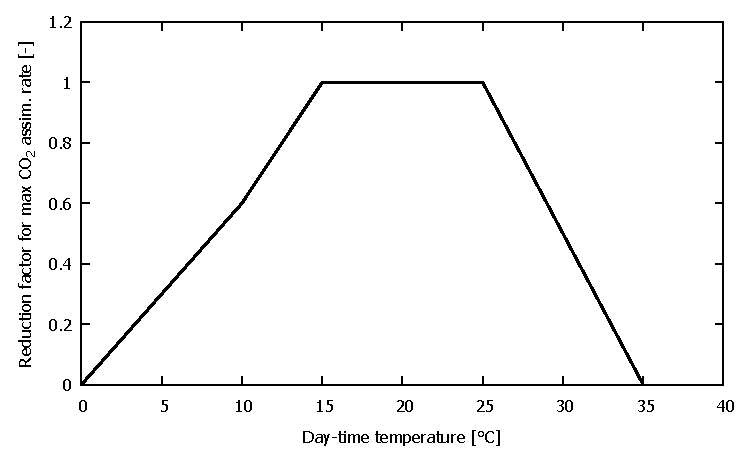
\includegraphics[width=140mm]{\FigDir/figure_TMPFTB.pdf}
	\caption{Reduction factor of the maximum leaf CO$_{{\rm 2}}$ assimilation rate as a function of
		average daytime temperature.}
	\label{fig:TMPFTB}
\end{figure}

\subsubsection{Nighttime temperature}
The gross CO$_{{\rm 2}}$ assimilation rate cannot exceed the maximum CO$_{{\rm 2}}$ assimilation rate. It
should also be noted that assimilation is an enzymatic process and such processes are
temperature dependent (Downes, 1970). However, there seems to be a considerable
adaption of the assimilation processes to fluctuating and varying temperatures (de Wit {\it et
	al.}, 1978). A wide temperature range for optimum photosynthetic performance under field
conditions is observed (Wardlaw, 1974). Low nighttime temperatures also affect the
assimilation. At night the assimilates, produced during daytime, are transformed into
structural biomass. This process is hampered by low temperature. If these low temperatures prevail 
for a several days, the assimilates accumulate in the plant and the assimilation rate diminishes 
and ultimately halts.

In the model, this temperature effect is accounted for by introducing a correction factor,
which should be multiplied with A$_{{\rm m}}$. This correction factor is a function of low minimum
temperature and is crop specific. An AFGEN table (acronym: {\bf TMNFTB}) is used to
describe this dependency.

As a measure for quantifying the effect of low minimum temperature, the seven day
running average of minimum temperature is used as the independent variable in the
AFGEN table (see also Appendix 2).

\begin{equation}
% eq 5.33
T _{low} ~=~\begin{array}{c}{i=7}  \\
\sum  \\
{i=1}\end{array}{\frac{\, T _{\min ,i} }{7}}
\end{equation}

Where:\\[5pt]
\begin{tabularx}{\textwidth}{llXr}
	T$_{{\rm min}}$  &:& Daily minimum temperature   &     [\degrees C]\\
	T$_{{\rm low}}$ &:& Seven day running average of minimum temperature    &    [\degrees C]\\
	i &:& Day    &    [-]
\end{tabularx}


\subsubsection{Photosynthesis in terms of CH$_{{\rm 2}}$O}
In the photosynthesis process, CO$_{{\rm 2}}$ is reduced to carbohydrates (CH$_{{\rm 2}}$O) using the energy
supplied by the absorbed light. The overall chemical reaction of this complex process is:

\begin{equation}
% equation 5.34
6\, CO_{2} ~+~ 6\, H_{2}O ~~ \underrightarrow{light} ~~ C_{6} H_{12} O_{6} ~+~ 6\, O_{2}
\end{equation}

or in simplified form:

\begin{equation}
% equation 5.35
CO_{2} ~+~ H_{2} O~~ \underrightarrow{light} ~~ CH_{2} O ~+~ O_{2}
\end{equation}

For each kg of CO$_{{\rm 2}}$ absorbed, 30/44 kg of CH$_{{\rm 2}}$O is formed, the numerical values
representing the molecular weights of CH$_{{\rm 2}}$O and CO$_{{\rm 2}}$ respectively.

\begin{equation}
% equation 5.36
R _{d}^{1} ~=~ A _{d}^{1} \,\,{\frac{30}{44}}
\end{equation}

Where:\\[5pt]
\begin{tabularx}{\textwidth}{llXr}
	R$^{{\rm 1}}$$_{{\rm d}}$ &:& Gross daily CH$_{{\rm 2}}$O assimilation rate 
	(not corrected for water stress) &   [kg ha$^{{\rm -1}}$ d$^{{\rm -1}}$]\\
	A$^{{\rm 1}}$$_{{\rm d}}$ &:& Gross daily CO$_{{\rm 2}}$ assimilation rate 
	(see eq. \ref{eq:5.11}) (corrected for low minimum temperature)   &    [kg ha$^{{\rm -1}}$ d$^{{\rm -1}}$]\\   
\end{tabularx}

As mentioned earlier, the gross daily CO$_{{\rm 2}}$ assimilation rate, A$^{{\rm 1}}$$_{{\rm d}}$, 
can be calculated by multiplying the total hourly instantaneous assimilation rate (eq. \ref{eq:5.31}) 
with the day length (eq. \ref{eq:AstroDaylength}). 


%\subsection{Reductions for water, oxygen and nutrient stress}
%\label{sec:PhotosynthesisReductionFactors}

\subsubsection{Water stress}
The calculated daily assimilation in CH$_{{\rm 2}}$O per ha will be reduced when crop transpiration
is reduced. The latter is caused by reduced water update by roots either due to water shortage or water 
surplus causing oxygen stress. In the model the effects of water stress on assimilation are related 
to the ratio of actual transpiration and potential transpiration (van Keulen \& Seligman, 1987).
The reduction factor for transpiration reduction can thus be calculated as.

\begin{equation}
\label{eq:5.37}
RF_{tra} ~=~ {\frac{T _{a} }{T _{p} }}
\end{equation}

Where:\\[5pt]
\begin{tabularx}{\textwidth}{llXr}
	$RF_{{\rm tra}}$ &:& Reduction factor for reduced transpiration rates   & [-]\\
	T$_{{\rm a}}$ &:& Actual transpiration   &     [cm d$^{{\rm -1}}$]\\
	T$_{{\rm p}}$ &:& Potential transpiration   &     [cm d$^{{\rm -1}}$]\\
\end{tabularx}

In \S \ref{sec:evapotranspiration} the calculation of the potential, T$_{{\rm p}}$, and actual 
the transpiration, T$_{{\rm a}}$, will be explained.

\section{Maintenance respiration}

Some of the carbohydrates formed are respired to provide energy for maintaining the
existing biostructures. The maintenance processes include resynthesis of degraded proteins
(especially enzymes) and maintenance of ionic gradients across cell membranes. The
higher the metabolic activity of the plant, the higher the maintenance costs (Penning de
Vries, 1975), probably due to a higher enzyme turnover and higher transport costs.

Maintenance respiration provides the energy for living organisms to maintain their
biochemical and physiological status. Through the reaction which is the reverse of CO$_{{\rm 2}}$
reduction in the CO$_{{\rm 2}}$ assimilation, the radiation energy which was fixed in the
photosynthetic process is released in a suitable form (ATP and NADPH):

\begin{equation}
% eq 5.38
CH _{2} O ~+~ O _{2} ~\longrightarrow~ CO _{2} ~+~ H _{2} O ~+~ energy
\end{equation}

This maintenance respiration consumes roughly 15 - 30\% of the carbohydrates produced
by a crop in a growing season (Penning de Vries {\it et al.}, 1979). This indicates the
importance of accurate quantification of this process in the model.

\subsection{Maintenance respiration as a function of the weight of dry matter}
The maintenance costs may be estimated on the basis of the quantities of proteins and
minerals present in the biomass and on crop metabolic activity, as presented by De Wit {\it et
	al.} (1978). This method, however, requires information on the nitrogen and mineral
contents of the vegetation.
Based on the results of this analysis, typical values for the maintenance coefficients of
various plant organs have been derived by Penning de Vries \& van Laar (1982).
In the model, these coefficients are used to calculate the maintenance requirements of the
crop. According to this approach the maintenance requirements are approximately 
proportional to the dry weights of the plant organs to be maintained: 

\begin{equation}
\label{eq:5.39}
R _{m,r} ~ = ~\begin{array}{c} {i=1}  \\
\sum  \\
{i=4}\end{array} \, c _{m,i} \, W _{i}
\end{equation}

Where:\\[5pt]
\begin{tabularx}{\textwidth}{llXr}
	R$_{{\rm m,r}}$ &:& Maintenance respiration rate at reference 
	temperature of 25 \degrees C &   [kg ha$^{{\rm -1}}$ d$^{{\rm -1}}$]\\
	c$_{{\rm m,i}}$ &:& Maintenance coefficient of organ i  & [kg kg$^{{\rm -1}}$ d$^{{\rm -1}}$]\\
	W$_{{\rm i}}$ &:& Dry matter weight organ i (see eq. \ref{eq:5.49})   &     [kg ha$^{{\rm -1}}$]\\
	i &:& Leaves (lv), storage organs (so), stems (st) or roots (rt)\\ 
\end{tabularx}

The maintenance coefficient of organ i, {\bf c$_{{\rm m,i}}$}, is crop dependent and should be provided by
the user. Acronyms used in the model: {\bf RML} (lv), {\bf RMO} (so), {\bf RMS} (st) and {\bf RMR} (rt).

In \S \ref{sec:DMpartitioning}, $\Delta$W$_{{\rm i}}$, the increase of the dry matter weight of 
organ i per time step, will be
discussed. Integration of $\Delta$W$_{{\rm i}}$ over the previous time steps yields the total dry matter
weight of organ i (dead and alive). Integration of the net increase of dry matter, $\Delta$Wn$_{{\rm i}}$,
(see eq. \ref{eq:5.48}) over the previous time steps yields the living dry matter weight of organ i
(see eq \ref{eq:5.49}).

\subsection{Dependency of the maintenance respiration on development stage}
The calculated maintenance respiration rate (eq. \ref{eq:5.39}) has to be corrected for senescence.
This correction factor is crop specific and is defined as a function of development stage. 
An AFGEN table (acronym: {\bf RFSETB}) with the development stage as
independent variable, is used to describe this dependency. The maintenance respiration
should be multiplied with this factor.  Note that differences in nitrogen contents in the different organs 
due to aging of the plant may cause differences in the maintenance coefficients. 

\subsection{Dependency of the maintenance respiration on temperature}
Higher temperatures accelerate the turnover rates in plant tissue and hence the costs of
maintenance. An increase in temperature of 10\degrees C increases maintenance respiration by a
factor of about 2 (Kase \& Catsky, 1984; Penning de Vries \& van Laar, 1982). However,
in order to be more flexible, in the model a variable {\bf Q$_{{\rm 10}}$} (acronym: {\bf Q10}) is introduced.
Q$_{{\rm 10}}$ is defined as the relative increase of the respiration rate per 10\degrees C temperature
increase. Q$_{{\rm 10}}$ should be provided by the user. The rate of the maintenance respiration at a
certain temperature, can be calculated with:

\begin{equation}
\label{eq:5.40}
R _{m,T} ~=~ R _{m,r} \, Q _{10}^{~~{\frac{T-T _{r} }{10}} }
\end{equation}

Where:\\[5pt]
\begin{tabularx}{\textwidth}{llXr}
	R$_{{\rm m,T}}$ &:& Maintenance respiration rate at 
	temperature T &    [kg ha$^{{\rm -1}}$ d$^{{\rm -1}}$]\\
	R$_{{\rm m,r}}$ &:& Maintenance respiration rate at reference 
	temperature of 25 \degrees C (see eq. \ref{eq:5.39})   &     [kg ha$^{{\rm -1}}$ d$^{{\rm -1}}$]\\
	Q$_{{\rm 10}}$ &:& Relative increase of the respiration rate
	per 10\degrees C temperature increase    &    [-]\\
	T &:& Average daily temperature    &     [\degrees C]\\
	T$_{{\rm r}}$ &:& Reference temperature {\small [=25 \degrees C in 
		the model]}    &    [\degrees C]\\
\end{tabularx}


For tropical species, the reference temperature may be 10\degrees C higher than for species from
temperate climates. The maintenance requirements of a crop are likely to be adapted to
the higher growth temperatures. However, in WOFOST 7.1 the reference temperature is
fixed at 25\degrees C for all crops.

As stated before, maintenance respiration rate depends on the amount of dry matter in the
various organs, the relative maintenance rate per organ and the temperature. It cannot
exceed the actual gross assimilation rate. It is assumed that the vegetation will not be
'self-consuming' in terms of carbohydrates. Actual gross assimilation rate minus 
maintenance respiration rate results in the amount of assimilates available for conversion into
structural material. When the crop ages, its metabolic activity and therefore its
maintenance requirements decreases. This effect could be accounted for by relating 
the maintenance coefficients to the N content of the tissues (van Keulen \& Seligman, 1987).


\section{Transpiration and evaporation}
\label{sec:evapotranspiration}

Transpiration, or the rate of water loss from the plants depends on the energy available
for vaporization, on the difference in vapor pressure between the plant and the surrounding 
air and on the resistance to water vapor diffusion from the stomatal cavity to the
atmosphere (van Keulen \& Seligman, 1987). Potential transpiration is the water loss from
a field crop which covers the soil completely and has an optimum supply of water from
the soil. 

\subsection{Evaporation and transpiration}
Potential evapotranspiration of a crop ET0 is the sum of potential transpiration T$_{{\rm m}}$ and
soil evaporation E0$_{{\rm s}}$.

\begin{equation}
\label{eq:6.2}
ET0 ~=~ E0_{s} ~+~ T_{m} 
\end{equation}

Where:\\[5pt]
\begin{tabularx}{\textwidth}{llXr}
	ET0 &:& Potential evapotranspiration rate (see \S 4.1.3) & [cm d$^{{\rm -1}}$]\\
	E0$_{{\rm s}}$ &:& Potential evaporation of a bare soil (see \S 4.1.3)  & [cm d$^{{\rm -1}}$]\\
	T$_{{\rm m}}$ &:& Maximum crop transpiration rate (see eq. 6.4)  & [cm d$^{{\rm -1}}$]\\
\end{tabularx}

For some crops the potential evapotranspiration can be higher than the Penman-Monteith
reference evapotranspiration. 
Therefore, in the model a correction factor, a so called  crop coefficient
(acronym: {\bf CFET}) is introduced to account for this effect. The Penman-Monteith evapotranspiration
should be multiplied by this crop coefficient (Feddes, 1978; Doorenbos \& Pruitt, 1977).
The evaporation is reduced due to the presence of vegetation, which intercepts the solar
energy and reduces the windspeed. The evaporation of the soil as a function of the leaf
area index (Goudriaan, 1977; Ritchie, 1972; 1971) can be estimated as:

\begin{equation}
\label{eq:6.3}
E0 _{s} ~=~ ET0 \cdot e^{-\kappa_{gb} \cdot LAI}
\end{equation}

Where:\\[5pt]
\begin{tabularx}{\textwidth}{llXr}
	E0$_{{\rm s}}$ &:& Potential bare soil evaporation  & [cm d$^{{\rm -1}}$]\\
	$\kappa$$_{{\rm gb}}$ &:& Extinction coefficient for global radiation  & [-]\\
	LAI &:& Leaf area index  & [ha ha$^{{\rm -1}}$]\\
\end{tabularx}

The potential transpiration rate can be calculated by combining equations \ref{eq:6.2} and 
\ref{eq:6.3}.

\begin{equation}
\label{eq:6.4}
T _{m} ~=~ ET0\, (1~-~e ^{-\kappa _{gb} \, LAI} )
\end{equation}

Where:\\[5pt]
\begin{tabularx}{\textwidth}{llXr}
	T$_{{\rm m}}$ &:& Maximum crop transpiration rate & [cm d$^{{\rm -1}}$]\\
	ET0 &:& Potential evapotranspiration rate & [cm d$^{{\rm -1}}$]\\
	$\kappa$$_{{\rm gb}}$ &:& Extinction coefficient for global radiation & [-]\\
	LAI &:& Leaf area index (see \S \ref{sec:growthofleaves}) & [ha ha$^{{\rm -1}}$]\\
\end{tabularx}

The extinction coefficient for global radiation can be estimated as a factor times the
extinction coefficient of diffuse radiation:

\begin{equation}
\label{eq:6.5}
\kappa_{gb} ~=~ 0.75\, \kappa_{df} 
\end{equation}

Where:\\[5pt]
\begin{tabularx}{\textwidth}{llXr}
	$\kappa_{{\rm gb}}$ &:& Extinction coefficient for global radiation & [-]\\
	$\kappa_{{\rm df}}$ &:& Extinction coefficient for diffuse light & [-]\\
\end{tabularx}

The maximum evaporation rate from a shaded water surface can be calculated in the same
way as equation \ref{eq:6.4}: 

\begin{equation}
\label{eq:6.6}
E_{w,\max } ~=~ E0_{w} \cdot e^{-\kappa_{gb} LAI}
\end{equation}

Where:\\[5pt]
\begin{tabularx}{\textwidth}{llXr}
	E$_{{\rm w,max}}$ &:& Maximum evaporation rate from a shaded water surface & 
	[cm d$^{{\rm -1}}$]\\
	E0$_{{\rm w}}$ &:& Potential evaporation rate from a water surface 
	(see \S \ref{sec:penman}) & [cm d$^{{\rm -1}}$]\\
	$\kappa$$_{{\rm gb}}$ &:& Extinction coefficient for global radiation & [-]\\
	LAI &:& Leaf area index & [ha ha$^{{\rm -1}}$]\\
\end{tabularx}

The maximum evaporation rate from a shaded bare soil surface can also be calculated in
the same way as in equation \ref{eq:6.4} and \ref{eq:6.6}:

\begin{equation}
\label{eq:6.7}
E_{s,\max } ~=~ E0 _{s} \,\,\, e ^{-\kappa  _{gb} LAI}
\end{equation}

Where:\\[5pt]
\begin{tabularx}{\textwidth}{llXr}
	E$_{{\rm s,max}}$ &:& Maximum evaporation rate from a shaded 
	soil surface & [cm d$^{{\rm -1}}$]\\
	E0$_{{\rm s}}$ &:& Potential evaporation rate from a bare soil 
	surface & [cm d$^{{\rm -1}}$]\\
	$\kappa$$_{{\rm gb}}$ &:& Extinction coefficient for total global radiation & [-]\\
	LAI &:& Leaf area index & [ha ha$^{{\rm -1}}$]\\
\end{tabularx}

\subsection{Reduction of the transpiration due to water stress}

For the potential yield level the actual transpiration rate is always equal to the maximum
transpiration rate, because sufficient water is available. The actual transpiration rate is
calculated from the maximum transpiration rate, taking into account reductions for
shortage or excess of water in the root zone. Water uptake by the roots depends on the
difference in potential between the water in the plant and in the soil, and on the resistance
to transport of moisture from the soil to the atmosphere (van Keulen \& Seligman, 1987).
In contrast to Feddes {\it et al}. (1978) not soil water potential, but soil water content is
chosen as the independent variable (Gollan {\it et al}., 1986; Schulze 1986).

Up to a point, the water potential in the plant can be adapted in order to maintain
potential transpiration. At what soil moisture content the transition from potential
transpiration to a transpiration deficit takes place, is difficult to quantify. In the model,
the actual transpiration for the water limited run is obtained by multiplying the potential
transpiration with a reduction factor. This reduction factor is defined as (van Diepen {\it et al}., 1988):

\begin{equation}
\label{eq:6.8}
R_{ws} ~=~{\frac{\theta_{t} ~-~ \theta  _{wp} }{ \ _{ws} ~-~ \theta_{wp} }}
\end{equation}

Where:\\[5pt]
\begin{tabularx}{\textwidth}{llXr}
	$R_{{\rm ws}}$ &:& Reduction factor for transpiration in case of
	water shortage & [-]\\
	$\theta_{{\rm t}}$ &:& Actual soil moisture content (see eq. 6.1 and 
	6.34) & [cm$^{{\rm 3}}$ cm$^{{\rm -3}}$]\\
	$\theta_{{\rm wp}}$ &:& Soil moisture content at wilting 
	point & [cm$^{{\rm 3}}$ cm$^{{\rm -3}}$]\\
	$\theta_{{\rm ws}}$ &:& Critical soil moisture & [cm$^{{\rm 3}}$ cm$^{{\rm -3}}$]\\ 
\end{tabularx}

The critical soil moisture content is defined as the quantity of stored soil moisture below
which water uptake is impaired and the crop begins to close its stomata. It is not a fixed
value. Restriction of water uptake due to water stress starts at a higher water content
when the potential transpiration rate is higher (Denmead \& Shaw, 1962). The critical
moisture content can be calculated as (van Diepen {\it et al}., 1988):

\begin{equation}
\label{eq:6.9}
\theta_{ws} ~=~ (1\, -\, p )\, (\theta_{fc} \, -\, \theta_{wp} )\, +\, \theta_{wp} 
\end{equation}

Where:\\[5pt]
\begin{tabularx}{\textwidth}{llXr}
	$\theta$$_{{\rm ws}}$ &:& Critical soil moisture content & [cm$^{{\rm 3}}$ cm$^{{\rm -3}}$]\\
	p &:& Soil water depletion fraction as a function 
	of pot. evapotranspiration & [cm$^{{\rm 3}}$ cm$^{{\rm -3}}$]\\
	$\theta$$_{{\rm fc}}$ &:& Soil moisture content at field capacity & [cm$^{{\rm 3}}$ cm$^{{\rm -3}}$]\\
	$\theta$$_{{\rm wp}}$ &:& Soil moisture content at wilting point & [cm$^{{\rm 3}}$ cm$^{{\rm -3}}$]\\
\end{tabularx}

The soil moisture content at field capacity, {\bf $\theta$$_{{\rm fc}}$} (acronym: {\bf SMFCF}), 
and the soil moisture content at wilting point, {\bf $\theta$$_{{\rm wp}}$} (acronym: {\bf SMW}), 
are soil specific and should be given by the user. Figure \ref{fig:TaTp_vs_soilmoisture} provides
a graphical overview of the reduction function for transpiration (e.g. $T_a/T_p$) as a 
function of soil moisture content.

The soil water depletion fraction, p, is 
a function of the potential evapotranspiration rate (for a closed canopy) and the crop group 
number. It is established in subroutine
{\bf SWEAF}. In literature, instead of the term soil water depletion fraction, also the 
expression easily available water is used. Easily available water is defined as the amount of
water between $\theta$$_{{\rm fc}}$ and $\theta$$_{{\rm wp}}$ which can be extracted from the root 
zone without reducing the
transpiration. Indicative p-values for the most important crops at different values of ET0
are presented in Table 6.1. The crop group number ranges from 1 (drought-sensitive) to 5
(drought-resistant). An example of a classification of the different crop groups is
presented in Table 6.2.

\begin{table}
	% Table 6.1
	\caption{Soil water depletion fraction (p) as a function of potential evapotranspiration 
		of a closed crop canopy for different crop groups (Doorenbos {\it et al}.,1978).}
	\label{tbl:soilwatdeplfraction}
	\begin{tabularx}{\textwidth}{Xrrrrrrrrr}
		\hline
		\multicolumn{10}{c}{Crop ET0 in cm d-1}\\
		\hline
		group$^{\rm *}$ & 0.2 & 0.3 & 0.4 & 0.5 & 0.6 & 0.7 & 0.8 & 0.9 & 1.0\\
		1 & 0.45 & 0.38 & 0.30 & 0.25 & 0.23 & 0.20 & 0.18 & 0.16 & 0.15\\
		2 & 0.60 & 0.50 & 0.43 & 0.35 & 0.30 & 0.28 & 0.25 & 0.23 & 0.20\\
		3 & 0.75 & 0.65 & 0.55 & 0.45 & 0.40 & 0.38 & 0.33 & 0.30 & 0.25\\
		4 & 0.85 & 0.75 & 0.65 & 0.55 & 0.50 & 0.48 & 0.43 & 0.38 & 0.35\\
		5 & 0.92 & 0.85 & 0.75 & 0.65 & 0.60 & 0.55 & 0.50 & 0.48 & 0.45\\
		\hline 
	\end{tabularx} 
\end{table}


\begin{table}
	% Table 6.2
	\caption{Example of crops in the different crop groups (Doorenbos {\it et al}., 1978).}
	\label{tbl:ExampleCropGroups}
	\begin{tabularx}{\textwidth}{lX}
		\hline
		Group no & Representative crop types\\
		\hline
		1 & leaf vegetables, strawberry\\     
		1-2 & cabbage, onion\\
		2 & clover, carrot, early tobacco\\     
		2-3 & banana, pepper\\
		3 & grape, pea, potato\\
		3-4 & bean, sunflower, tomato, water melon, grass\\
		4 & citrus, groundnut, pineapple\\
		4-5 & alfalfa cotton, tobacco, cassava, sweet potato, grains\\
		5 & olive, safflower, sorghum, soybean, sugarcane\\
		\hline
	\end{tabularx}
\end{table}

The soil water depletion fraction for very high values of potential evapotranspiration of a
closed canopy can be as low as 0.10. For very low values of potential evapotranspiration
of a closed canopy this fraction can be as high as 0.96.
Note that it is possible that the reduction factor R$_{{\rm ws}}$ (eq. \ref{eq:6.8}) might obtain 
values higher
than unity and lower than zero for certain values of p and $\theta$$_{{\rm t}}$. Since this does not make
any sense, in the model the highest possible value for R$_{{\rm ws}}$ is set to unity and the lowest
possible value is set to zero.
An empirical formula can be used to calculate the fraction of easily available soil water,
yielding identical values as the ones given in the Table \ref{tbl:soilwatdeplfraction} 
(van Diepen {\it et al}., 1988).

\begin{equation}
\label{eq:6.10}
p~={\frac{~1}{ \alpha _{p} ~+~ \beta _{p} ~ET0}} ~-~ 0.10\, (\, 5~-~No _{cg} \, )
\end{equation}

Where:\\[5pt]
\begin{tabularx}{\textwidth}{llXr}
	p &:& Fraction of easily available soil water  & [cm$^{{\rm 3}}$ cm$^{{\rm -3}}$]\\
	$\alpha$$_{{\rm p}}$ &:& Regression constant {\small (=0.76 van Diepen et al., 1988)}  & [-]\\
	$\beta$$_{{\rm p}}$ &:& Regression constant {\small (=1.5 van Diepen et al., 1988)}  & [d cm-$^{{\rm 1}}$]\\
	ET0 &:& Potential evapotranspiration rate  & [cm d$^{{\rm -1}}$]\\
	No$_{{\rm cg}}$ &:& Crop Group number {\small (=1 to 5, Doorenbos et al., 1978)}  & [-]\\
\end{tabularx}

Note that crop group number, {\bf No$_{{\rm cg}}$} (acronym: {\bf DEPNR}) is input in the model and should
be provided by the user.

For crop group 1 and 2 this estimate is not very accurate and an additional correction is
applied to reproduce the table values correctly (van Diepen {\it et al}., 1988):

\begin{equation}
%eq 6.11
p~=~p~+~{\frac{ET0 ~-~ 0.6}{No _{cg} \, (\, No _{cg} ~+~3\, )}}
\end{equation}

Where:\\[5pt]
\begin{tabularx}{\textwidth}{llXr}
	where p &:& Fraction of easily available soil water  & [cm$^{{\rm 3}}$ cm$^{{\rm -3}}$]\\
	ET0 &:& Potential evapotranspiration rate  & [cm d$^{{\rm -1}}$]\\
	No$_{{\rm cg}}$ &:& Crop Group number {\small (=1 to 5, Doorenbos et al., 1978)}  & [-]\\
\end{tabularx}

\subsection{Reduction of the transpiration due to oxygen stress}
The transpiration rate of the plants can also be reduced when the root zone is completely
saturated. Root systems which have been developed in aerobic soils do not have airducts
and degenerate within several days when anaerobic conditions (waterlogging) are imposed
(Penning de Vries {\it et al}., 1989). Flooding quickly depletes the O$_{{\rm 2}}$ in the soil and root cells
disintegrate when their metabolic activities are hampered by oxygen depletion. For
detailed information on the physiological effects of excess water on a crop see Jackson
and Drew (1984).

Reduction in transpiration occurs when the actual soil moisture content exceeds the
critical soil moisture content for aeration. The critical soil moisture content for aeration
can be calculated as:

\begin{equation}
\label{eq:6.12}
\theta_{air} ~=~ \theta_{\max} ~-~\theta_{c} 
\end{equation}

Where:\\[5pt]
\begin{tabularx}{\textwidth}{llXr}
	$\theta$$_{{\rm air}}$ &:& Critical soil moisture content for aeration & [cm$^{{\rm 3}}$ cm$^{{\rm -3}}$]\\
	$\theta$$_{{\rm max}}$ &:& Soil porosity & [cm$^{{\rm 3}}$ cm$^{{\rm -3}}$]\\
	$\theta$$_{{\rm c}}$ &:& Critical air content & [cm$^{{\rm 3}}$ cm$^{{\rm -3}}$]\\
\end{tabularx}

The soil porosity, {\bf $\theta$$_{{\rm max}}$} (acronym: {\bf SMO}) and the critical soil air 
content, {\bf $\theta$$_{{\rm c}}$} (acronym:{\bf CRAIRC}), are soil specific and should 
be provided by the user. 

In the model, maximum reduction is reached after four successive days of anaerobic
conditions. In reality however, this period depends on the development stage and on the
species. If at the fifth successive day oxygen shortage occurs the reduction remains the
same as on the fourth day. The reduction factor for the transpiration rate due to oxygen
shortage can be calculated as (van Diepen, personal communication):

\stepcounter{equation}
\begin{align}
\label{eq:6.13a-b}
R_{os,\max } &= \frac{ \theta  _{\max } ~-~ \theta  _{t} }{\theta _{\max } ~-~ \theta  _{air} } \subeqn  \\
R_{os} &= 1 - \frac{No _{d} }{4} \, (\, 1\, -\, R _{os,\max } \, ) ~~~ with~~ No_{d} ~\le ~ 4 \subeqn
\end{align}

Where:\\[5pt]
\begin{tabularx}{\textwidth}{llXr}
	R$_{{\rm os,max}}$ &:& Maximum reduction factor due to oxygen shortage & [-]\\
	R$_{{\rm os}}$ &:& Reduction factor due to oxygen shortage & [-]\\
	$\theta$$_{{\rm air}}$ &:& Critical soil moisture content for aeration 
	& [cm$^{{\rm 3}}$ cm$^{{\rm -3}}$]\\
	$\theta$$_{{\rm max}}$ &:& Soil porosity & [cm$^{{\rm 3}}$ cm$^{{\rm -3}}$]\\
	$\theta$$_{{\rm t}}$ &:& Actual soil moisture content (see eq. \ref{eq:6.34}) 
	& [cm$^{{\rm 3}}$ cm$^{{\rm -3}}$]\\
	No$_{{\rm d}}$ &:& Number of successive days with oxygen stress & [-]\\
\end{tabularx}

For crops which roots develop airducts, like for example rice, and for crops grown on
perfectly drained land, the reduction factor for oxygen shortage equals unity. If this ratio
is less then unity, the actual transpiration rate is reduced proportionally.

Usually, in freely draining soils oxygen stress does not play any role. It may occur when
the critical soil moisture content for aeration is greater than the soil moisture content at
field capacity and when the subsoil is very slowly permeable. In case of groundwater
influence, oxygen shortage may occur regularly. However, the process of transpiration
reduction due oxygen shortage is poorly parametrized and therefore values for the
reduction factor are rather speculative. 

\subsection{Actual transpiration}
As a result of water excess and/or water shortage the reduction factor for the transpiration rate can be
calculated as:

\begin{equation}
\label{eq:6.14}
RF_{tra} = R_{ws} \,\, R_{os}
\end{equation}

Figure \ref{fig:TaTp_vs_soilmoisture} provides an overview of the ratio $\frac{T_a}{T_p}$ as
a function of soil moisture level $\theta$. 


\begin{figure}[p]
	\centering
	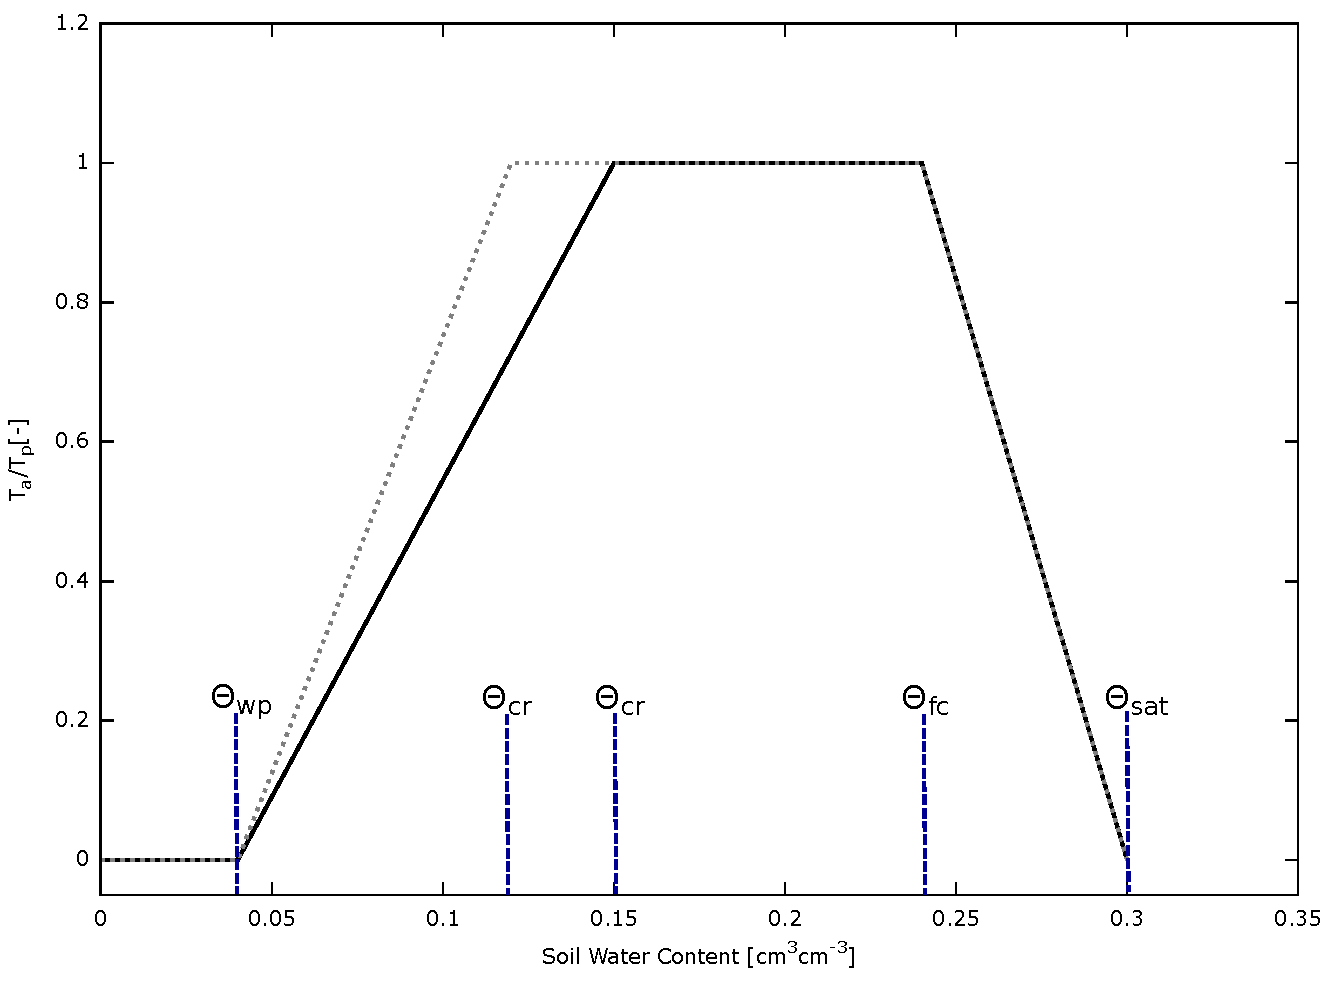
\includegraphics[width=120mm]{\FigDir/figure_FeddesTrapezoid.pdf}
	\caption{The relation between soil water content, $\theta$, and Ta/Tp for a crop/soil combination. 
		$\theta_{{\rm wp}}$, $\theta_{cr}$, $\theta_{{\rm wp}}$ and $\theta_{{\rm sat}}$ represent the water
		 content of the soil at wilting point, the critical point for potential transpiration, field capacity 
		 and saturation, respectively. The dashed line represents either a more drought resistant species under
		 the same field conditions, or the same species under a lower evaporative demand, caused by different
		 weather conditions (Penning de Vries et al., 1989; van Laar et al., 1992)}
	\label{fig:TaTp_vs_soilmoisture}
\end{figure}

\section{Growth}

The amount of the absorbed CH$_{{\rm 2}}$O that remains after correction and reduction of the
gross CO$_{{\rm 2}}$ assimilation rate (e.g. the net assimilation rate) is available to be 
converted into dry matter. Growth, 
in fact is the increase in dry matter ignoring its water content. The net assimilation rate
is thus simply the difference between the gross actual assimilation rate and the losses due to
maintenance respiration:

\begin{equation}
	R_{n} = R_{d} ~-~ R _{m,T} 
\end{equation}

Where:\\[5pt]
\begin{tabularx}{\textwidth}{llXr}
	R$_{{\rm n}}$ &:& Net assimilation rate   &     [kg ha$^{{\rm -1}}$ d$^{{\rm -1}}$]\\
	R$_{{\rm d}}$ &:& Actual daily CH$_{{\rm 2}}$O assimilation rate (see eq. \ref{eq:5.37})   &   
	[kg ha$^{{\rm -1}}$ d$^{{\rm -1}}$]\\
	R$_{{\rm m,T}}$ &:& Maintenance respiration rate at 
	temperature T (see eq. \ref{eq:5.40})   &     [kg ha$^{{\rm -1}}$ d$^{{\rm -1}}$]\\
\end{tabularx}

As it is assumed that the maintenance respiration cannot be larger than the actual gross 
assimilation rate, the net assimilation rate will be zero or larger.

The pattern of dry matter distribution over the various plant organs is closely related to
the development stage of the crop. Development is defined as progression in the successive 
phenological stages. It is characterized by the formation rate of the various vegetative
and reproductive organs and their order of appearance. However, before the growth rates
of the different organs can be computed, first the growth respiration has to be taken into account.

\subsection{Growth respiration}

The conversion of the net assimilate rate into structural plant material requires energy which is
called 'growth respiration' in WOFOST.
In this conversion process of the glucose molecules, CO$_{{\rm 2}}$ and
H$_{{\rm 2}}$O are released. This is a partial combustion of glucose to provide energy required in
the various biochemical pathways. Hence, biosynthesis of the various structural compounds can 
be considered a process of cut and paste, the scraps representing the weight
lost in growth respiration.
Each structural compound is formed along a distinct, non crop-specific pathway.
Following these reactions, the weight of glucose required to produce a unit of the
compound can be calculated (Penning de Vries {\it et al.}, 1974). The transport costs of the
molecules are included. Two active passages of membranes are assumed. Each active
passage requires 1 ATP, which is provided by respiring $^{{\rm 1}}$/$_{{\rm 3}}$$_{{\rm 8}}$ molecule of glucose.

The assimilates required to produce a unit weight of a certain plant organ can now be
calculated from its chemical composition and the assimilate requirements of the various
chemical compounds. Storage organs (grains, tubers, etc.) vary to much in composition
among species for one general value of their assimilate requirements to be given. The
conversion efficiency represents the inverse of the assimilate requirement.

At higher temperatures the conversion processes are accelerated, but the pathways are
identical (Spitters {\it et al.} 1989). Hence, the assimilate requirements do not vary with
temperature. 

At higher temperatures the conversion processes are accelerated, but the pathways are
identical (Spitters {\it et al.} 1989). Hence, the assimilate requirements do not vary with
temperature. The growth respiration rate can then be calculated as:

\begin{equation}
\label{eq:5.41}
R _{g} ~=~ R _{d} ~-~ R _{m,T} 
\end{equation}

Where:\\[5pt]
\begin{tabularx}{\textwidth}{llXr}
	R$_{{\rm g}}$ &:& Growth respiration rate   &     [kg ha$^{{\rm -1}}$ d$^{{\rm -1}}$]\\
	R$_{{\rm d}}$ &:& Actual daily CH$_{{\rm 2}}$O assimilation rate (see eq. \ref{eq:5.37})   &   
	[kg ha$^{{\rm -1}}$ d$^{{\rm -1}}$]\\
	R$_{{\rm m,T}}$ &:& Maintenance respiration rate at 
	temperature T (see eq. \ref{eq:5.40})   &     [kg ha$^{{\rm -1}}$ d$^{{\rm -1}}$]\\
\end{tabularx}

As explained, conversion into dry matter costs energy, therefore a conversion factor is
defined. This factor depends on the conversion efficiency of assimilates and on the
partitioning factors of the different organs. The dry matter is multiplied with this overall
conversion efficiency factor to calculate the dry matter increase. The conversion 
efficiency of carbohydrates into structural plant material is calculated as a weighted average
of the efficiencies for the various plant organs.

\begin{equation}
\label{eq:5.42}
C _{e} ~={\frac{~1}{
		\begin{array}{c}
		{i=3}  \\
		\sum  \\
		{i=1}
		\end{array} {pc_{i}}/{C_{e,i}} \cdot (1-pc_{rt} ) + {pc_{rt}}/{C_{e,rt}} 
}}
\end{equation}

Where:\\[5pt]
\begin{tabularx}{\textwidth}{llXr}
	C$_{{\rm e}}$ &:& Conversion efficiency factor of assimilates, total crop  &   
	[kg kg$^{{\rm -1}}$]\\
	C$_{{\rm e,i}}$ &:& Conversion efficiency factor of the assimilates 
	of a specified organ  &      [kg kg$^{{\rm -1}}$]\\
	pc$_{{\rm i}}$ &:& Partitioning factor of organ i   &
	[kg kg$^{{\rm -1}}$]\\
	i &:& Leaves (lv), storage organs (so), stems (st)\\
	rt &:& roots\\
\end{tabularx}

The conversion efficiency factor for the assimilates of a specified organ, {\bf C$_{{\rm e,i}}$}, is crop
specific and should be given by the user. Acronyms used in the model: {\bf CVL} (leaves), {\bf CVO}
(storage organs), {\bf CVR} (roots) and {\bf CVS} (stems).

The dry matter growth rate of the total crop can be calculated as:

\begin{equation}
% eq 5.43
\Delta W~=~ C_{e} \cdot R_{n} 
\end{equation}

Where:\\[5pt]
\begin{tabularx}{\textwidth}{llXr}
	$\Delta$W &:& Dry matter growth rate total crop   &
	[kg ha$^{{\rm -1}}$ d$^{{\rm -1}}$]\\
	C$_{{\rm e}}$ &:& Conversion efficiency factor of assimilates,
	total crop (see eq. \ref{eq:5.42})    &    [kg kg$^{{\rm -1}}$] \\
	R$_{{\rm n}}$ &:& Net assimilation rate (see \ref{eq:5.41})   &
	[kg ha$^{{\rm -1}}$ d$^{{\rm -1}}$]\\
\end{tabularx}

\subsection{Dry matter partitioning}
\label{sec:DMpartitioning}

In WOFOST the dry matter is partitioned over the 4 parts of the
plant. In the model, total dry matter growth is partitioned according to fixed distribution
factors, defined as a function of development stage. Dry matter is first partitioned
between shoots and roots. 

\stepcounter{equation}
\begin{align}
% eqn 5.44a,b
\Delta W_{rt} &= pc_{rt} \cdot \Delta W   \subeqn  \\
\Delta W_{sh} &= (1 - pc_{rt}) \Delta W \subeqn
\end{align}


Where:\\[5pt]
\begin{tabularx}{\textwidth}{llXr}
	$\Delta$W &:& Dry matter growth rate total crop   &
	[kg ha$^{{\rm -1}}$ d$^{{\rm -1}}$]\\
	$\Delta$W$_{{\rm rt}}$ &:& Dry matter growth rate roots    &
	[kg ha$^{{\rm -1}}$ d$^{{\rm -1}}$]\\
	$\Delta$W$_{{\rm sh}}$ &:& Dry matter growth rate shoots    &
	[kg ha$^{{\rm -1}}$ d$^{{\rm -1}}$]\\
	pc$_{{\rm rt}}$ &:& Partitioning factor of roots    &
	[kg kg$^{{\rm -1}}$]\\
\end{tabularx}

The growth rate of leaves, stems and storage organs is simply the product of the dry
matter growth rate of the shoots and the fraction allocated to these organs.

\begin{equation}
\label{eq:5.45}
\Delta W_{i} ~=~ pc_{i} \cdot \Delta W_{sh} 
\end{equation}

Where:\\[5pt]
\begin{tabularx}{\textwidth}{llXr}
	$\Delta$W$_{{\rm i}}$ &:& Dry matter growth rate of organ i &
	[kg ha$^{{\rm -1}}$ d$^{{\rm -1}}$]\\
	$\Delta$W$_{{\rm sh}}$ &:& Dry matter growth rate of shoots   &
	[kg ha$^{{\rm -1}}$ d$^{{\rm -1}}$]\\
	pc$_{{\rm i}}$ &:& Partitioning factor of organ i    &
	[kg kg$^{{\rm -1}}$]\\
	i &:& Leaves (lv), storage organs (so), stems (st)
\end{tabularx}

The partitioning factors, {\bf pc$_{{\rm i}}$}, are a function of development stage and are crop specific. In
the model, the dependency is described using AFGEN tables with the development stage
as the independent variable (see Appendix 2). Acronyms used in the model: {\bf FLTB} (lv),
{\bf FOTB} (so), {\bf FRTB} (rt) and {\bf FSTB} (st).

At any development stage the following relation must be valid, if not, the simulation will
be stopped (see also fig. 5.6):

\begin{equation}
% eq 5.46
pc_{lv} + pc_{st} + pc_{so} = 1
\end{equation}

Where:\\[5pt]
\begin{tabularx}{\textwidth}{llXr}
	pc$_{{\rm i}}$ &:& Partitioning factor of organ i   &
	[kg kg$^{{\rm -1}}$]\\
	i &:& Leaves (lv), storage organs(so), stems (st)
\end{tabularx}

\begin{figure}[p]
	% fig 5.6
	\centering
	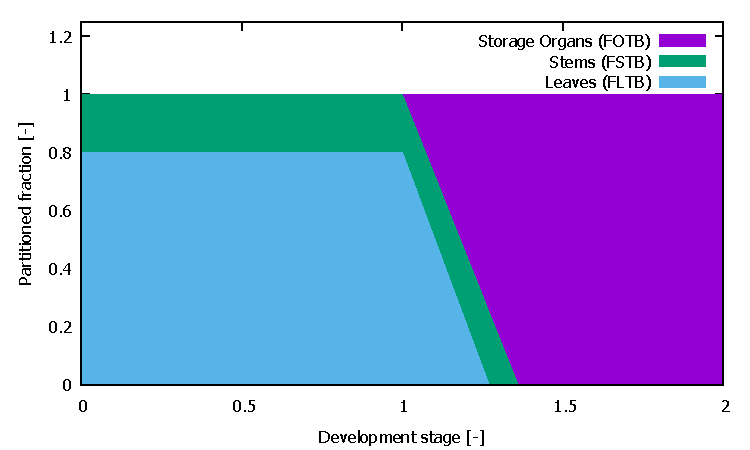
\includegraphics[width=120mm]{\FigDir/figure_PARTITIONING.pdf}
	\caption{Example of the partitioning factors for potato of the different organs as a function of development stage.}
	\label{fig:partitioning}
\end{figure}

The actual gross CO$_{{\rm 2}}$ assimilation rate has to be identical to the amount of structural plant
material produced plus the amounts used for maintenance respiration and conversion (see
figure 5.1). The carbon balance has to be zero. 

\begin{equation}
\label{eq:5.47}
0 = {\frac{R_{d} - R_{m,T} - R_{g} \big( pc_{rt} + (pc_{lv} + pc_{st} + pc_{so}) \cdot (1 - pc_{rt}) \big) }{R_d}}  
\end{equation}

Where:\\[5pt]
\begin{tabularx}{\textwidth}{llXr}
	R$_{{\rm g}}$ &:& Growth respiration rate (see eq. \ref{eq:5.41})   &
	[kg ha$^{{\rm -1}}$ d$^{{\rm -1}}$]\\
	R$_{{\rm d}}$ &:& Actual daily CH$_{{\rm 2}}$O assimilation rate (see eq. \ref{eq:5.37})   &
	[kg ha$^{{\rm -1}}$ d$^{{\rm -1}}$]\\
	R$_{{\rm m,T}}$ &:& Maintenance respiration rate (see eq. \ref{eq:5.40})   &
	[kg ha$^{{\rm -1}}$ d$^{{\rm -1}}$]\\
	pc$_{{\rm i}}$ &:& Partitioning factor of organ i    &
	[kg kg$^{{\rm -1}}$]\\
	i &:& Leaves (lv), storage organs (so), stems (st), roots (rt)\\
\end{tabularx}

As mentioned earlier, it is assumed that maintenance respiration can not exceed the actual
gross assimilation rate. However, in case the daily CH$_{{\rm 2}}$O assimilation rate comes close to
zero, this might happen and therefore simulation should be stopped. Introducing a
division by R$_{{\rm d}}$ in the carbon check (eq. \ref{eq:5.47}) will identify the occurrence of such an
event.

%\subsection{Growth and leaf senescence  }
%\label{sec:5.4.5}
%
%As is explained in paragraph \ref{sec:DMpartitioning}, the growth rate of a leaves, stems or 
%storage organs is obtained by
%multiplying the growth rate of the shoot by the fraction allocated to that organ.
%Its total dry biomass (dead and alive) is obtained by integrating this growth rate over
%time. Taking the death rate of the different organs into account, the integration of the net
%increase of dry matter, $\Delta$Wn$_{{\rm i}}$, (see eq. \ref{eq:5.48}) over the previous time steps 
%yields the living dry matter weight of organ i (see eq. \ref{eq:5.49}).
%
%This approach of the partitioning of dry matter is descriptive, as the distribution keys are
%defined as a function of the development stage of the crop only. The influence of
%environmental factors could be included by applying modification factors to these keys,
%depending on temperature, water and nutrient status of the crop, and its reserve level
%(Loomis {\it et al.}, 1979; van Keulen \& Seligman, 1987). In the WOFOST model, however,
%this is not applied. Some more attention is paid to the crop growth by introducing a death
%rate for leaves, roots and stems. Death rate is a function of the development stage of the
%plant and is crop and organ specific.

\subsection{Growth of stems, roots and storage organs}

In the model, the death rate of the storage organs is considered to be zero. For the roots
and the stems increase in living biomass can be easily determined as the growth rate
minus death rate. This yields the net growth rate (eq. \ref{eq:5.48}). The death rate is crop
specific and is defined as the daily amount of the living biomass which no longer
participates in the plant processes. The death rate of stems and roots is considered to be a
function of development stage. This dependency is described using an
AFGEN table with the development stage as the independent variable (see also Appendix
2). The death rate of leaves is more complicated. Leaf senescence due to shading (high
LAI), water stress and also due to exceedance of the life span should be accounted for.

The net growth rate of the stems and roots can described by:

\begin{equation}
\label{eq:5.48}
\Delta Wn _{i~} =~\,\,\Delta W _{i~} -~ {\rm \dag } _{i} \,\, W _{i} 
\end{equation}

Where:\\[5pt]
\begin{tabularx}{\textwidth}{llXr}
	$\Delta$Wn$_{{\rm i}}$ &:& Net dry matter growth rate of organ i   &
	[kg ha$^{{\rm -1}}$ d$^{{\rm -1}}$]\\
	$\Delta$W$_{{\rm i}}$ &:& Dry matter growth rate of organ i (see eq. \ref{eq:5.45})   &
	[kg ha$^{{\rm -1}}$ d$^{{\rm -1}}$]\\
	W$_{{\rm i}}$ &:& Dry matter weight organ i  &
	[kg ha$^{{\rm -1}}$]\\
	\dag $_{{\rm i}}$ &:& Death rate organ i   &
	[kg kg$^{{\rm -1}}$ d$^{{\rm -1}}$]\\
	i &:& Stems (st), roots (rt)\\
\end{tabularx}

The death rates of stems and roots are crop specific and should be provided by the user.
A dependency of the development stage is assumed. AFGEN tables (acronym: {\bf RDRRTB}
(rt), {\bf RDRSTB} (st)) with the development stage as the independent variable are used to
describe this dependency.

Although the process which describes the death rate of leaves is more complicated than
the calculation of the death rate of stems and roots, the calculation to establish the total
dry weight of living leaves is the same as the computation of the dry matter weight of
stems and roots. The total dry matter weight of living leaves, stems and roots can be
found by integration over time of the net dry matter growth, $\Delta$Wn$_{{\rm i}}$, yields 
the dry matter.

\begin{equation}
\label{eq:5.49}
W _{t,i} ~=~W _{t-1\, ,\, i} ~+~\Delta Wn _{i} \,\Delta t
\end{equation}

Where:\\[5pt]
\begin{tabularx}{\textwidth}{llXr}
	W$_{{\rm i,t}}$ &:& Dry matter weight organ i at time step t   &
	[kg ha$^{{\rm -1}}$]\\
	$\Delta$Wn$_{{\rm i}}$ &:& Net dry matter growth rate of organ i   &
	[kg ha$^{{\rm -1}}$ d$^{{\rm -1}}$]\\
	$\Delta$t &:& Times step   &
	[d]\\
	i &:& Stems (st), roots (rt), leaves (lv)\\
\end{tabularx}

The equation \ref{eq:5.49} is recursive. In the model, the initial values of the dry weight of the
various organs are calculated. An initial value for the total dry weight of the crop
(acronym: {\bf TDWI}) should be provided by the user. This value is multiplied by the
partioning factors, pc$_{{\rm i}}$, at emergence, yielding the initial values of dry weight of the
various organs.

\subsection{Growth of leaves}
\label{sec:growthofleaves}
The area of green leaves is the major determinant for light absorption and photosynthesis
of the crop. Under optimal conditions, light intensity and temperature are the environmental factors influencing the rate of leaf area expansion. Light intensity determines the
rate of photosynthesis and hence the supply of assimilates to the leaves.

Temperature affects the rates of cell division and extension (Ng \& Loomis, 1984; Sheehy
{\it et al.}, 1980; Acock {\it et al.}, 1978). During the early stages of crop growth, temperature is
the overriding factor. The rate of leaf appearance and final leaf size are constrained by
temperature through its effect on cell division and extension, rather than by the supply of
assimilates (Hunt, 1982; Causton \& Venus, 1981; van Dobben, 1962). The growth curve
in the early stage has an exponential form. Some unpublished field data have shown that
the exponential model should be restricted to the situation where the development stage, 
D$_{{\rm s,t}}$ $<$ 0.3 and LAI $<$ 0.75 (see also eq. \ref{eq:5.4}). In the model, however, it is assumed that
the exponential growth rate of the leaf area index is valid until the source-limited increase
of the leaf area index equals the exponential growth rate.

The growth rate of the leaf area index per time step in the early, exponential growth
stage, can be calculated as:

\begin{equation}
% eq:5.50
L _{Exp,t} ~=~LAI _{{t~RL~T}_{e}}
\end{equation}

Where:\\[5pt]
\begin{tabularx}{\textwidth}{llXr}
	L$_{{\rm Exp,t}}$ &:& Growth rate of the leaf area index at time step t
	during exponential growth stage   &    [ha ha$^{{\rm -1}}$ d$^{{\rm -1}}$]\\
	LAI$_{{\rm t}}$ &:& Leaf area index at time step t    &
	[ha ha$^{{\rm -1}}$]\\
	RL &:& Maximum relative increase of leaf area index   &
	[\degrees C$^{{\rm -1}}$ d$^{{\rm -1}}$]\\
	T$_{{\rm e}}$ &:& Daily effective temperature (see 5.2c)   &
	[\degrees C]\\
\end{tabularx}

In theory, the maximum relative increase of the leaf area index, {\bf RL}, is a function of
effective temperature. For a relative wide range of temperatures {\bf RL} responds more or
less linearly to temperature (Hunt {\it et al.}, 1985; Causton \& Venus, 1981; van Dobben,
1962). In the model however, a fixed value per crop type is assumed (acronym: 
{\bf RGRLAI}). This value should be given by the user.

The accumulated leaf area index at time step t during the exponential growth stage can be
described as:

\begin{equation}
\label{eq:5.51}
LAI _{t~} =~LAI _{t-1} ~+~L _{Exp\, ,\, t} ~\Delta t
\end{equation}

Where:\\[5pt]
\begin{tabularx}{\textwidth}{llXr}
	L$_{{\rm Exp,t}}$ &:& Growth rate of the leaf area index at time step t
	during exponential growth stage    &    [ha ha$^{{\rm -1}}$ d$^{{\rm -1}}$]\\
	LAI$_{{\rm t}}$ &:& Leaf area index at time step t   &
	[ha ha$^{{\rm -1}}$]\\
	$\Delta$t &:& Time step   &    [d]
\end{tabularx}

The equation\ref{eq:5.51} is recursive. In the model, {\bf LAI$_{{\rm t}}$} is initialized by 
setting the starting
value equal to the leaf area index at emergence (acronym: {\bf LAIEM}). The leaf area index
at emergence is crop specific and should be provided by the user.

During the development of the crop, leaf area expansion is increasingly restricted by
assimilate supply (i.e. source limited increase). Branching and tillering generate an
increasing number of sites per plant, where leaf initiation can take place. As mentioned
earlier, in the model it is assumed that the exponential growth rate of leaf area index will
continue until it equals the source limited growth rate of the leaf area index.

The growth rate of the leaf area index at time step t during the source limited growth 
stage can be described by:

\begin{equation}
\label{eq:5.52}
L _{Sc,t} ~=~\Delta Wn _{lv} ~S _{la} 
\end{equation}

Where:\\[5pt]
\begin{tabularx}{\textwidth}{llXr}
	L$_{{\rm Sc,t}}$ &:& Growth rate of the leaf area index at time step t
	during the source limited growth stage    &
	[ha ha$^{{\rm -1}}$ d$^{{\rm -1}}$]\\
	$\Delta$Wn$_{{\rm lv}}$ &:& Net dry matter growth of leaves at time step t    &
	[kg ha$^{{\rm -1}}$ d$^{{\rm -1}}$]\\
	S$_{{\rm la}}$ &:& Specific leaf area at time step t   &
	[ha kg$^{{\rm -1}}$]\\
\end{tabularx}

The net dry matter growth of leaves, $\Delta$Wn$_{{\rm lv}}$, can be found by subtracting the weight of
leaves which died during the current time step from the dry matter growth of leaves,
$\Delta$W$_{{\rm lv}}$. This process will be described later in more detail in this paragraph.

The specific leaf area, {\bf S$_{{\rm la}}$} (acronym: {\bf SLATB}), is defined as the increase of the leaf area
of the crop per kg weight increase of the living leaves. S$_{{\rm la}}$ is crop specific and a function
of the development stage (see figure 8). In the model this dependency is described using
an AFGEN table with the development stage as the independent variable (see also
Appendix 2).

The accumulated leaf area index at time step t during the source limited growth stage can
be described as:

\begin{equation}
\label{eq:5.53}
LAI _{t~} =~LAI _{t-1} ~+~L _{Sc\, ,\, t} ~\Delta t
\end{equation}

Where:\\[5pt]
\begin{tabularx}{\textwidth}{llXr}
	L$_{{\rm Sc,t}}$ &:& Growth rate of the leaf area index at time step t
	during the source limited growth stage     &   [ha ha$^{{\rm -1}}$ d$^{{\rm -1}}$]\\
	LAI$_{{\rm t}}$ &:& Leaf area index at time step t     &
	[ha ha$^{{\rm -1}}$]\\
	$\Delta$t &:& Time step    &    [d]\\
\end{tabularx}

The equation \ref{eq:5.53} is recursive. In the model, {\bf LAI$_{{\rm t}}$} is initialized by 
taking the fraction of initial biomass (acronym: {\bf TWDI}) partitioned to the leaves and 
multiply at with the specific leaf area at the current DVS. Note that in older versions of
WOFOST a specific leaf area index at emergence (acronym: {\bf LAIEM}) was used which should 
be provided by the user. However, the use of {\bf LAIEM} is deprecated.

In the model, however, the accumulated leaf area cannot be calculated directly. The leaf
area index has to be corrected for leaf senescence which occurred during the current time
step. The leaf senescence can be caused by physiological ageing, water stress and/or high
leaf area index (i.e. mutual shading). Later in this text, more attention will be paid to
these effects.

In order to correct for leaf senescence, the specific leaf area of each time step, S$_{{\rm la}}$, the
growth of the dry matter weight of leaves per time step, $\Delta$W$_{{\rm lv}}$ and the physiological age,
P$_{{\rm age}}$ (see eq. \ref{eq:5.57}), have to be stored in three different arrays. These arrays are organized
as follows: the first element of the arrays represents the most recent age class (or time
step) and the last element of the arrays represents the oldest age class (or time step). It
should be clear that the position of an element in the arrays represents its age class, in
time steps. The dry matter weight of the leaves, which have died during the current time
step, has to be. subtracted from the growth of dry matter weight per time step. One array
contains thus the net dry matter growth of the leaves per time step, $\Delta$Wn$_{{\rm lv}}$. 
The procedure which describes this process will be explained later in this text. 

After the correction for leaf senescence, the accumulated leaf area can be established. The
net dry matter weight of the leaves, $\Delta$Wn$_{{\rm lv,}}$  in the remaining and new leaf classes is
multiplied with the specific leaf areas (see eq. \ref{eq:5.52}) to get the growth rate of the leaf area
index of the living leaves per age class. Multiplication with $\Delta$t and summation over the
classes (eq. \ref{eq:5.53}) yields the total leaf area index. The green area index of the stems and
the storage organs is added to this amount. The total dry matter weight of living leaves
can be found in a similar way by using equation \ref{eq:5.49}.

\begin{figure}[p]
	%Fig. 5.8   
	\centering
	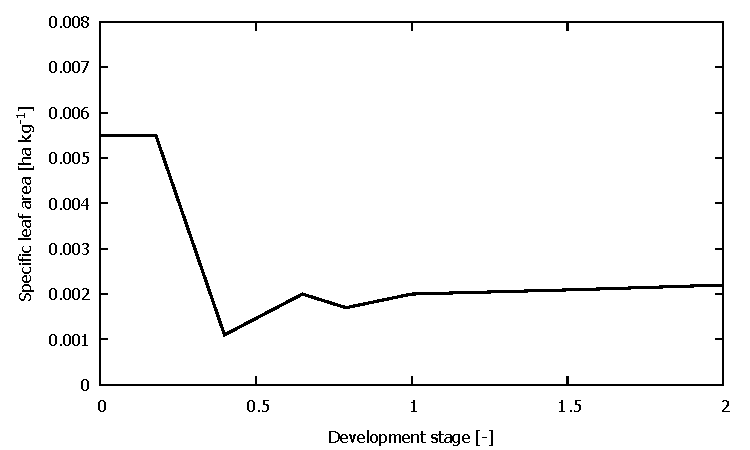
\includegraphics[width=120mm]{\FigDir/figure_SLATB.pdf}
	\caption{Specific leaf area as a function of development stage (example for rice).}
	\label{fig:SpecificLeafArea}
\end{figure}

As is mentioned earlier, the green area index of the stems and storage organs, may absorb
a substantial amount of radiation. Therefore it should be added to the total leaf area
index. The green area index of these organs can be calculated by:

\begin{equation}
% eq:5.54
GAI_{i} ~=~SS _{i} W _{i} 
\end{equation}

Where:\\[5pt]
\begin{tabularx}{\textwidth}{llXr}
	GAI$_{{\rm i}}$ &:& Green area index of organ i    &
	[ha ha$^{{\rm -1}}$]\\
	SS$_{{\rm i}}$ &:& Specific green area of organ i    &
	[ha kg$^{{\rm -1}}$]\\
	W$_{{\rm i}}$ &:& Dry matter organ i (see eq. \ref{eq:5.49})    &
	[kg ha$_{{\rm -1}}$]\\
	i &:& Stems (st), storage organs (so)\\
\end{tabularx}

The specific green area of stems (acronym: {\bf SSA}) and storage organs (acronym: {\bf SPA}) are
crop specific and should be provided by the user. The specific storage organ area is also
known as the specific pod area.

Special attention should be paid to the fact that during the exponential growth stage, the
specific leaf is not established. Therefore, during this period, for each time step, the
specific leaf area has to be calculated according to:

\begin{equation}
% eq:5.55
S_{\exp,t} ~=~ {\frac{L_{\exp,t}}{\Delta W_{lv} }}
\end{equation}

Where:\\[5pt]
\begin{tabularx}{\textwidth}{llXr}
	S$_{{\rm exp,t}}$ &:& Specific leaf area at time step t during the 
	exponential growth stage    &     [ha kg$^{{\rm -1}}$]\\
	$\Delta$W$_{{\rm lv}}$ &:& Dry matter increase of leaves (see eq. \ref{eq:5.45})   &
	[kg ha$_{{\rm -1}}$ d$^{{\rm -1}}$]\\
	L$_{{\rm \exp,t}}$ &:& Growth rate of the leaf area index at time step t
	during exponential growth stage (see eq. \ref{eq:5.51})   &
	[ha ha$^{{\rm -1}}$ d$^{{\rm -1}}$]\\
\end{tabularx}

In de model, it is assumed that senescence does not occur during the exponential growing
stage. This means that $\Delta$W$_{{\rm lv}}$ can be used in stead of the net dry matter 
growth, $\Delta$Wn$_{{\rm lv}}$.

\subsection{Death of leaves (senescence)}
As stated before, leaf senescence is more complicated. Senescence refers to the loss of
capacity to carry out essential physiological processes and to the loss of living biomass.
The fundamental processes involve physiological ageing and protein breakdown. These
processes are difficult to quantify. Leaves are assumed to die when they have completed
their life cycle. The dying rate may be accelerated as a result of drought stress or of
mutual shading.

{\it physiologic ageing}\\
Leaves die due to exceedance of the life span for leaves (i.e. physiologic ageing). Life
span is defined as the maximum time in days a leaf can live at a constant temperature of
35\degrees C. Life span is crop specific. The concept of lifespan is compatible with a definition
in terms of temperature sum as given by Gallagher (1979).
The physiologic ageing factor per time step can be calculated as:

\begin{equation}
% eq:5.56
f _{rai} ~=~{\frac{ T~-~T _{b\, ,\, age} }{35~-~ T _{b\, ,\, age} }}
\end{equation}

Where:\\[5pt]
\begin{tabularx}{\textwidth}{llXr}
	f$_{{\rm rai}}$ &:& Physiologic ageing factor for leaf age increase   &
	[-]\\
	T &:& Daily (average) temperature   &
	[\degrees C]\\
	T$_{{\rm b,age}}$ &:& Lower threshold temperature for physiologic ageing   &
	[\degrees C]\\
\end{tabularx}

The lower threshold temperature for physiologic ageing, {\bf T$_{{\rm b,age}}$} (acronym: {\bf TBASE}), is
crop specific and should be provided by the user. The integral of the physiologic ageing
factor over time yields the physiologic age. 

\begin{equation}
\label{eq:5.57}
P _{age,t} ~=~ P _{age,t-1} ~+~f_{rai} \Delta t
\end{equation}

Where:\\[5pt]
\begin{tabularx}{\textwidth}{llXr}
	P$_{{\rm age,t}}$ &:& Physiologic age at time step t & [d]\\
	f$_{{\rm rai}}$ &:& Physiologic ageing factor for leaf age increase & [-]\\
	$\Delta$t &:& time step & [d]\\
\end{tabularx}

Leaves may attain the age defined by the crop specific life span (acronym: {\bf SPAN}).
However, as is mentioned earlier, they can not exceed it. In the model the ages of the
leaf classes are checked. The first class younger than the defined life span becomes the
oldest class. Note that death of old leaves takes place after ageing, being the result of the
daily shifting from one leaf class to the next (Johnson \& Thornley, 1983). In this way,
the life time of leaves is the maximum number of days that a leaf class contributes to the
LAI and to photosynthesis.

{\it Death rate due to water stress}\\
The potential death rate of leaves due to water stress can be calculated as:

\begin{equation}
% eq:5.58
\Delta W_{d}^{1} ~=~ W_{lv} \, (\, 1\, -\,{\frac{T _{a} }{T _{p} }} \, )\, {\rm \dag } _{\max ,lv} 
\end{equation}

Where:\\[5pt]
\begin{tabularx}{\textwidth}{llXr}
	$\Delta$W$^{{\rm 1}}$$_{{\rm d}}$ &:& Potential death rate of leaves due to water stress   &
	[kg  ha$^{{\rm -1}}$ d$^{{\rm -1}}$]\\
	\dag $_{{\rm max,lv}}$ &:& Maximum relative death rate of leaves due to
	water stress   &     [kg kg$^{{\rm -1}}$ d$^{{\rm -1}}$]\\
	W$_{{\rm lv}}$ &:& Dry matter weight of the leaves (see eq. \ref{eq:5.49})  &
	[kg ha$^{{\rm -1}}$]\\
	T$_{{\rm a}}$ &:& Actual transpiration (see \S \ref{sec:evapotranspiration})    &
	[cm d$^{{\rm -1}}$]\\
	T$_{{\rm p}}$ &:& Potential transpiration (see \S \ref{sec:evapotranspiration})   &
	[cm d$^{{\rm -1}}$]\\
\end{tabularx}

The maximum relative death rate of leaves due to water stress, {\bf \dag $_{{\rm max,lv}}$} 
(acronym: {\bf PERDL}) is crop specific and should be provided by the user.

{\it Death rate due to high leaf area index}\\
Leaf senescence also occurs due to high leaf area index (i.e. mutual shading). A relative
death rate due to self$-$shading is defined which increases linearly from zero at a certain,
critical leaf area index, to its maximum value at twice this critical leaf area index. Typical
values for the maximum relative death rate and the critical LAI are 0.03 d$^{{\rm -1}}$ and 4 
ha ha$^{{\rm -}{1}}$, respectively (Spitters {\it et al.} 1989).

The potential death rate of leaves due to high LAI can be calculated as:

\begin{equation}
% eq:5.59
\Delta W_{d}^{2} ~=~ W_{lv} \cdot 0.03 \cdot {\frac{LAI - LAI_c}{LAI_c}}
\end{equation}

Where:\\[5pt]
\begin{tabularx}{\textwidth}{llXr}
	$\Delta$W$^{{\rm 2}}$$_{{\rm d}}$ &:& Potential death rate of leaves due to 
	high LAI   &    [kg ha$^{{\rm -1}}$ d$^{{\rm -1}}$]\\
	W$_{{\rm lv}}$ &:& Dry matter weight of the leaves  &  [kg ha$^{{\rm -1}}$]\\
	LAI &:& Leaf area index   &    [ha ha$^{{\rm -1}}$]\\
	LAI$_{{\rm c}}$ &:& Critical leaf area index   &     [ha ha$^{{\rm -1}}$]\\
\end{tabularx}

The critical leaf area index, LAI$_{{\rm c}}$, can be computed by:

\begin{equation}
% eq:5.60
LAI_{c} = {\frac{3.2}{\kappa_{df} }}
\end{equation}

Where:\\[5pt]
\begin{tabularx}{\textwidth}{llXr}
	LAI$_{{\rm c}}$ &:& Critical leaf area index    &    [ha ha$^{{\rm -1}}$]\\
	$\kappa$$_{{\rm df}}$ &:& Extinction coefficient for 
	the diffuse radiation flux   &    [-]\\
\end{tabularx}

The last term of the right hand side of the equation 5.59 must be between 0 and 0.03. A 
value lower than 0 will be set to 0 and a value higher than 0.03 will be set to 0.03. In the
model, the highest value of the two calculated potential death rates of leaves, 
$\Delta$W$^{{\rm 1}}$$_{{\rm d}}$ and $\Delta$W$^{{\rm 2}}$$_{{\rm d}}$, is selected 
for further calculations of the reduction of dry matter weight increase,
per time step of the leaf classes, as is will be explained now. 

The weight of leaves which have died during the current time step, can be calculated by
multiplying the death rate (due to water stress and/or high LAI), with the time step.

\begin{equation}
% eq:5.61
W_{d} = \max(\Delta W_{d}^{1} , \Delta W_{d}^{2})\cdot \Delta t
\end{equation}

Where:\\[5pt]
\begin{tabularx}{\textwidth}{llXr}
	W$_{{\rm d}}$ &:& Weight of leaves that have died during 
	current time step    &    [kg ha$^{{\rm -1}}$]\\
	$\Delta$W$^{{\rm 1}}$$_{{\rm d}}$ &:& Potential death rate of leaves due 
	to water stress   &      [kg ha$^{{\rm -1}}$ d$^{{\rm -1}}$]\\
	$\Delta$W$^{{\rm 2}}$$_{{\rm d}}$ &:& Potential death rate of leaves due to 
	high LAI   &     [kg ha$^{{\rm -1}}$ d$^{{\rm -1}}$]\\
	$\Delta$t &:& Time step    &    [d]\\
\end{tabularx}

The weight of the leaves which have died, W$_{{\rm d}}$, is subtracted from the weight of the oldest
leaf class. If there is only one class the result should be positive. When more leaf classes
exist, the oldest leaf class may be emptied completely, the remainder is subtracted from
the next leaf class. Emptying the oldest leaf class goes on, until the original amount is
dissipated completely and the remaining amount of leaves remains positive. All leaves are
shifted every time step (daily) to the next class.

\subsection{Root growth}
\label{sec:rootgrowth}

Growth of roots in terms of depth is implemented in a straightforward way in WOFOST. 
The model assumes that at the start of the crop simulation, the crop has an initial rooting 
depth which is usually set to 10 cm. After initialization, the crop grows with a fixed daily 
increase in rooting depth until either a crop-specific maximum depth or a soil-defined maximum 
depth is reached. In versions of WOFOST that implement a shallow groundwater table, the 
increase in root depth will also cease if the roots are within 10cm of the groundwater 
table and the crop cannot form airducts. WOFOST does not define a root density profile 
and assumes that plant roots can subtract water equally from the entire rooted layer.

Growth of roots in terms of biomass follows the same logic as other plant organs in that
the roots receive a fraction of the net daily assimilates based on the partitioning 
fraction to roots for that day. Similar to stems, death of root material depends on 
the development stage through a relative death rate that causes a fraction of the 
roots to die after a certain development stage.

In the model there is no relationship between the amount of biomass partitioned to the roots 
and the increase of the depth of the roots, with the exception that the increase in root
depth will cease if there is no partitioning of biomass to roots anymore. Also there is 
no impact of environmental conditions (such as drought) on root growth.

In the model, root growth is implemented in a straightforward way. One needs to specify
the following crop and soil specific parameters:
\begin{itemize}
	\item Initial rooting depth, {\bf RD$_{{\rm i}}$} (acronym: {\bf RDI});
	\item Maximum rooting depth determined by the crop, {\bf RD$_{{\rm crop}}$} (acronym: {\bf RDMCR});
	\item Maximum daily increase in rooting depth, {\bf RR$_{{\rm max}}$} (acronym: {\bf RRI});
	\item Maximum rooting depth determined by the soil, {\bf RD$_{{\rm soil}}$} (acronym: {\bf RDMSOL}).
\end{itemize}

The daily increase of the rooting depth is a function of development stage and is crop
specific. The root growth can be calculated as:

\begin{equation}
% eq:5.62
\Delta RD~=~RR_{\max} \cdot \Delta t
\end{equation}

Where:\\[5pt]
\begin{tabularx}{\textwidth}{llXr}
	$\Delta$RD &:& Increase of the rooting depth   &   [cm]\\
	RR$_{{\rm max}}$ &:& Maximum daily increase in rooting depth  &  [cm d$^{{\rm -}{1}}$]\\
	$\Delta$t &:& Time step   &  [d]\\
\end{tabularx}

In the model it is assumed that the extension growth of the roots continues until the
maximum rooting depth is reached. The rooting depth can be established by:

\begin{equation}
% eq:5.63
RD _{t~} =~RD _{t-1} ~+~\Delta RD
\end{equation}

Where:\\[5pt]
\begin{tabularx}{\textwidth}{llXr}
	RD$_{{\rm t}}$ &:& Rooting depth at time step t   &  [cm]\\
	$\Delta$RD &:& Increase of the rooting depth    & [cm]\\
\end{tabularx}

In the model, the maximum rooting depth is established by taking the lowest value of the\\
maximum rooting depth determined by the crop, RD$_{{\rm crop}}$ and the maximum rooting depth
determined by the soil, RD$_{{\rm soil}}$. It is assumed that the maximum rooting depth is 
always equal or higher than the initial rooting depth.


\section{Crop variables}

The crop species are characterized by a set of parameters and functions. In the following
sub sections the estimated values, derived from experimental data, found in literature will
be discussed in some detail.

\subsection{Distribution and absorption of light in the canopy} 

The radiation flux, incident on a leaf, is partly absorbed and partly scattered. Scattering
consists of reflection and transmission. Species differ in the optical properties of their
leaves. In the model, a value of 0.20 is used for the scattering coefficient of individual 
leaves for PAR.

The light distribution within the canopy is characterized by the extinction coefficient ($\kappa$).
As a reference, the situation is considered where the leaves show a spherical angle
distribution (i.e. as if they were placed on the surface area of a sphere), and are 
distributed randomly within the canopy volume. Assuming the above scattering coefficient of
0.20, the theoretical value of the extinction coefficient for the diffuse radiation flux is
0.72 (Goudriaan, 1977). Actual values, however, can deviate substantially from this
theoretical value. Crops with more erect leaves have lower $\kappa$ values, whereas crops with
more prostrate leaves show higher values of $\kappa$. 

In the model, a spherical leaf angle
distribution is assumed. Alternative distributions can easily be implemented using the
procedure described by Goudriaan (1988). A clustered distribution of leaves increases
mutual shading, resulting in reduced light absorption and hence a lower value for $\kappa$.
However, especially in dicotyledons, new leaves are formed, preferably in gaps within the
canopy, thus increasing the value of $\kappa$. In the model, an actual value for the extinction
coefficient for diffuse radiation is used. The ratio between this actual value and the above
theoretical value is used as a cluster factor. The various extinction coefficients and the
fraction sunlit leaf area are multiplied by this factor.

Light absorption by organs other than leaves results in a calculated extinction coefficient
which is too high, if the measured extinction is related to leaf area only. If light 
absorption and assimilation by these organs are important, as for ears and panicles in cereals,
these processes should be accounted for explicitly in the model; e.g. by treating them as
light competing assimilators. This is also necessary for other factors, such as foliar
diseases, that affect the photosynthetic capacity of the leaves and are distributed
non$-$uniformly over canopy depth.

Typical values of $\kappa$ are 0.4 to 0.7 for monocotyledons and 0.65 to 1.1 for broad leaved
dicotyledons (Monteith, 1969). The extinction coefficient can be estimated from 
measurements of PAR above and below a canopy with a known LAI, making sure that PAR is
measured rather than total global radiation. The extinction coefficient for total radiation is
about $\frac{2}{3}$ that of PAR. 

The extinction coefficient has to be measured under a uniform overcast sky. Direct
radiation has to be avoided as the solar elevation determines the extinction coefficient for
direct radiation. In the morning all direct radiation will be absorbed and scattered in the
top layer of the canopy because of path length. At noon, direct radiation will penetrate
further in the canopy. If measurements have to be taken at a clear sky, a board can be
used to shade the light measurement instrument. Otherwise, the average extinction
coefficient over the day has to be calculated or the value has to be corrected for solar
elevation. Light extinction can be measured by comparing radiation intensity above and
below the canopy using a lightbar. From the LAI and the measured light extinction, the
extinction coefficient for the diffuse flux can be calculated. When global radiation is
measured the extinction coefficient for the diffuse flux will be about $\frac{2}{3}$ of the extinction
coefficient calculated for global radiation, because absorption of near the infrared
radiation by the canopy is less efficient.

An important factor which may confound the interpretation of measurements, is the light
absorption by other organs than leaves. In the calculation of the extinction coefficient for
diffuse light, from measurements, this effect should be accounted for.

\subsection{Photosynthesis-light response of individual leaves} 

The response of leaf photosynthesis to light intensity is characterized by its slope at low
light intensity ($\epsilon$) and its maximum rate at light saturation (A$_{{\rm m}}$). With respect to the
photosynthetic pathway, three groups of species can be identified: C$_{{\rm 3}}$ and C$_{{\rm 4}}$ species and
CAM plants. Lists of C$_{{\rm 4}}$ species have been published by Downton (1975) and
Raghavendra \& Das (1978).   

At a leaf temperature of 20\degrees C, both C$_{{\rm 3}}$ and C$_{{\rm 4}}$ species have an initial 
light use efficiency of approximately 12.5 $\mu$g CO$_{{\rm 2}}$ J$^{{\rm -1}}$ absorbed PAR or 0.45 kg 
CO$_{{\rm 2}}$ ha$^{{\rm -}{1}}$ leaf h$^{{\rm -}{1}}$ (J m$^{{\rm 2}}$ S$^{{\rm -}{1}}$)$^{{\rm -}{1}}$
(Ehleringer \& Pearcy, 1983). In C$_{{\rm 3}}$ species, $\epsilon$ decreases with increasing temperature due
to accelerated photo-respiration. This temperature effect is relatively small: $\epsilon$ changes by
about 1\% with each change of 1\degrees C in temperature (Farquhar {\it et al.}, 1980; Ehleringer,
1978; Leverenz \& \"{O}quist, 1987). In C$_{{\rm 4}}$ species, $\epsilon$ is not affected by temperature because
photo-respiration is suppressed in the C$_{{\rm 4}}$ pathway. 

Among both C$_{{\rm 3}}$ and C$_{{\rm 4}}$ species, there
is hardly any variation in (Ehleringer \& Pearcy, 1983). However, when $\epsilon$ is expressed per
unit of incident PAR, instead of per unit of absorbed PAR, apparent differences may
occur, due to differences in the absorption coefficient of the leaves (Hunt {\it et al.}, 1985).
Yellowing of leaves results in increased reflection and transmission and, therefore, in an
apparent decrease of $\epsilon$.  

Measured values of the gross assimilation rate of leaves at light saturation (A$_{{\rm m}}$) show a
large variation. The main sources of variation are differences in measurement conditions
of temperature and ambient CO$_{{\rm 2}}$ concentration, differences in physiological and 
anatomical properties of the leaves as a result of differences in leaf age and pre$-$treatment, and
variation among species and cultivars.

The influence of temperature on the rate of leaf photosynthesis is described in the model
by multiplying the value of A$_{{\rm m}}$ by a temperature$-$dependent factor. The relationship
between temperature and Am is based on Versteeg \& van Keulen (1986). Various
reaction types are distinguished according to crop species and habitat.

The photosynthetic capacity of the leaves is affected by the preceding conditions of
radiation and temperature to which they were exposed: leaves adapt their photosynthetic
capacity to the environment. Therefore, A$_{{\rm m}}$ shows a seasonal course, which correlates
with the time course of radiation and temperature (Parsons \& Robson, 1981). This
adaptation may be mimicked by using a seven$-$day running average of the value of A$_{{\rm m}}$
which has been adjusted for the environmental conditions (Schapendonk \& Gaastra, 1984;
Acock {\it et al.}, 1978). A consequence of this adaptation is that the photosynthetic 
characteristics of leaves of plants grown in climate rooms, are not representative for plants grown
in the field.

The photosynthetic capacity of a leaf is also affected by its age: A$_{{\rm m}}$ reaches a maximum
shortly after full expansion of the leaf, followed by a gradual decline with ageing
(Rawson {\it et al.}, 1983; Dwyer \& Stewart, 1986). Differences in photosynthetic capacity of
the leaves are closely related to their nitrogen content, whether these variations are due to
age, growing conditions or fertilizer application (van Keulen \& Seligman, 1987). Leaves

lower in the canopy have a lower photosynthetic capacity because they are older and are
adapted to lower radiation levels (Acock {\it et al.}, 1978; Williams, 1985). They also have
lower nitrogen concentrations. The value of A$_{{\rm m}}$ used in the model, refers to the
photosynthetic capacity of full$-$grown leaves at the top of the canopy, as these leaves
absorb most of the radiation. Effects of canopy senescence are introduced by a multiplication 
factor which is a function of development stage.

The photosynthetic capacity of leaves varies with crop species and cultivar. The coefficient of
variation in A$_{{\rm m}}$ among genotypes within a species is of the order of 5$-$10\%
(Spitters \& Kramer, 1986). Species can be grouped according to C$_{{\rm 3}}$ and C$_{{\rm 4}}$ types.
Characteristic values range from 15$-$50 kg CO$_{{\rm 2}}$ ha$^{{\rm -}{1}}$ leaf h$^{{\rm -}{1}}$ 
for C$_{{\rm 3}}$ species and from 40-90
kg CO$_{{\rm 2}}$ ha$^{{\rm -1}}$ h$^{{\rm -1}}$ for C$_{{\rm 4}}$ species, depending on leaf 
N concentration and temperature (Spitters {\it et al.}, 1986). Other values mentioned, 
range from 10$-$50 kg CO$_{{\rm 2}}$ ha$^{{\rm -}{1}}$ leaf h$^{{\rm -}{1}}$ for
C$_{{\rm 3}}$ species and from 10-90 kg CO$_{{\rm 2}}$ ha$^{{\rm -1}}$ h$^{{\rm -1}}$ 
for C$_{{\rm 4}}$ species (Goudriaan, 1982; van Keulen \&
Seligman, 1987). Species from ruderal habitats show higher values than species from
shaded habitats. In the model, estimates of A$_{{\rm m}}$ must be used, which are found by fitting
the exponential function [equation \ref{eq:5.23}] to data of gross photosynthesis of individual
leaves. Such estimates may deviate from the measured values of photosynthetic efficiency
at low light and photosynthesis at light saturation. If no firmly based value of A$_{{\rm m}}$ is
available, a value of 40 kg CO$_{{\rm 2}}$ ha$^{{\rm -1}}$ h$^{{\rm -}{1}}$ for C$_{{\rm 3}}$ 
species and 70 kg CO$_{{\rm 2}}$ ha$^{{\rm -1}}$ h$^{{\rm -1}}$ for C$_{{\rm 4}}$
species is, in general, a reasonable estimate.

\subsection{Respiration} 

Respiration is usually measured as CO$_{{\rm 2}}$ evolution in the absence of light energy. This
dark respiration can be partitioned into growth and maintenance respiration; estimation
procedures being reviewed by Amthor (1984). Standard values for maintenance coefficients are 
0.03 for leaves, 0.015 for stems and 0.01 for roots (Spitters {\it et al.}, 1989). For
tropical crops lower values are used: 0.02 for the leaves and 0.01 for the other plant
organs (Penning de Vries {\it et al.}, 1989). As mentioned previously, these coefficients are
affected by temperature, nitrogen content and mineral content of the plant tissue, and by
the metabolic activity of the crop.

Measured rates of dark respiration of full$-$grown leaves, showed a large variation among
species and among cultivars (M.J. de Kock, AB-DLO, Wageningen, unpubl.). The
maintenance coefficients applied in the model are not based on conclusive evidence. This
introduces a significant uncertainty in simulating the rate of crop growth, especially when
the standing biomass is large compared to the current rate of photosynthesis, as at the end
of the growth period.   


